% !TEX program = xelatex
% =============================================================================
%  MOSAICS Studio: all-atom natural-move Monte Carlo on modern additive
%  force fields in the browser
%
%  F. B. Omage and P. Minary
%
%  Assembly shell. Section text lives in sections/*.tex. The two tables that
%  carry measured numbers, tables/systems.tex and tables/matrix.tex, are
%  written by make_tables.py from the committed JSON and are not edited by
%  hand. Figures are produced by the scripts beside them in figures/.
%
%  Build:  tectonic -X compile main.tex        (also fine under pdflatex)
%  The bibliography is a hand-written thebibliography environment so that
%  no BibTeX run is needed; every entry was checked against the
%  publisher-deposited Crossref record at the DOI given.
% =============================================================================
\documentclass[11pt,a4paper]{article}

\usepackage[margin=22mm,top=24mm,bottom=26mm]{geometry}
\usepackage{iftex}
\ifxetex
  \usepackage[defaultsups]{newtxtext}
  \usepackage{newtxmath}
  \setsansfont{texgyreheros}[Extension=.otf,UprightFont=*-regular,BoldFont=*-bold,ItalicFont=*-italic,BoldItalicFont=*-bolditalic,Scale=0.90]
\else
  \usepackage[T1]{fontenc}
  \usepackage[utf8]{inputenc}
  \usepackage[defaultsups]{newtxtext}
  \usepackage{newtxmath}
  \usepackage[scaled=0.90]{helvet}
\fi
\emergencystretch=1.5em
\usepackage{microtype}
\usepackage{amsmath}
\usepackage{booktabs}
\usepackage{graphicx}
\usepackage{xcolor}
\usepackage{caption}
\usepackage{subcaption}
\usepackage{siunitx}
\usepackage{titlesec}
\usepackage{authblk}
\usepackage{enumitem}
\usepackage{url}
\usepackage[colorlinks=true,allcolors={blue!55!black}]{hyperref}

\graphicspath{{figures/}}
\sisetup{group-separator={,},group-minimum-digits=4,detect-all}
\captionsetup{font=small,labelfont={bf,sf},labelsep=period,justification=justified}
\titleformat{\section}{\sffamily\bfseries\large}{\thesection}{0.8em}{}
\titleformat{\subsection}{\sffamily\bfseries}{\thesubsection}{0.8em}{}
\titleformat{\paragraph}[runin]{\bfseries}{}{0em}{}[.]
\titlespacing{\paragraph}{0pt}{6pt plus 2pt}{0.6em}
\setlength{\parskip}{0pt}
\setlist{nosep,leftmargin=1.4em}
\renewcommand\Authfont{\normalsize}
\renewcommand\Affilfont{\small\itshape}
\setlength{\affilsep}{2pt}
\urlstyle{same}

\newcommand{\studio}{MOSAICS Studio}
\newcommand{\kcal}{kcal/mol}

\title{\sffamily\bfseries\Large \studio{}: all-atom natural-move Monte Carlo on modern
additive force fields in the browser}

\author[1]{Folorunsho Bright Omage}
\author[1,*]{Peter Minary}
\affil[1]{Department of Computer Science, University of Oxford, Wolfson Building,
Parks Road, Oxford OX1 3QD, United Kingdom}
\affil[*]{Corresponding author: \texttt{peter.minary@cs.ox.ac.uk}}

\date{8 September 2026}

\begin{document}
\maketitle

\begin{abstract}
\noindent
\input{sections/abstract}
\end{abstract}

\section{Introduction}
\label{sec:introduction}

The conformational changes that matter biologically are collective: a loop
folding over an occupied active site, two domains rotating against one another
so that a duplex groove opens far enough to admit a protein side chain. Tens to
hundreds of atoms move together, over microseconds or longer, and molecular
dynamics reaches that regime slowly for a structural reason rather than an
implementation one. The integrator has to resolve the fastest motion present,
which is the stretch of a bond to hydrogen, so the step is a few femtoseconds
and a microsecond costs of order $10^{9}$ of them \cite{dror2012microscope};
trajectories long enough to watch a domain rearrange or a small protein fold
have generally required purpose-built hardware
\cite{shaw2010anton,lindorfflarsen2011folding}. The usual response is to bias
the dynamics, by umbrella sampling \cite{torrie1977umbrella}, replica exchange
\cite{sugita1999remd}, metadynamics \cite{laio2002metadynamics} or one of their
relatives \cite{bernardi2015enhanced}, which buys sampling at the price of
either many replicas or a collective variable that has to be guessed before the
run starts.

Natural-move Monte Carlo attacks the same problem from the other side. Instead
of displacing every atom by a small amount and repeating, it displaces a
structurally meaningful group of atoms by a large amount, once. The user
partitions the molecule into groups (a chain, a domain, a helical arm, a
backbone segment between two anchors) and nests those groups in a hierarchy. A
move picks a group and applies a rigid rotation and translation to it, or turns
torsions inside it, leaving everything outside where it was. That breaks the
covalent geometry at the two boundaries of the group, and the break is repaired
by a stochastic chain-closure algorithm that finds the alternative closed
geometries, chooses among them and reports the weight needed to keep the
Metropolis test exact \cite{minary2010chainclosure}. The composite proposal is
then accepted or rejected against the Boltzmann factor in the usual way
\cite{sim2012naturalmoves}. The granularity is the point: one accepted move can
shift a whole segment along the path a hinge would take, and the nesting lets
one proposal act at the scale of a domain and the next at the scale of a sugar
pucker. Nothing has to be chosen in advance about \emph{where} the system should
go, only about which parts of it are plausibly rigid. The approach has predicted
sequence-dependent nucleosome occupancy without training on occupancy data
\cite{minary2014nucleosome}, refined structures into single-particle EM and
cryo-EM densities \cite{zhang2012multiscale,chang2020rnacryoem}, modelled
epigenetic marks on DNA \cite{krawczyk2018epigenetic}, and followed peptide
dissociation from MHC class~I \cite{knapp2016pmhc}.

All-atom Monte Carlo on additive force fields is not itself new, and this paper
does not claim it. CAMPARI samples all-atom polypeptide and nucleic-acid models
under the ABSINTH implicit-solvent model and under imported additive parameter
sets \cite{vitalis2009mcmethods}; MCPRO and BOSS were built around OPLS-AA
\cite{jorgensen2005mcpro}; ProtoMS computes binding free energies under AMBER
and OPLS parameters \cite{protoms-software}; and Cassandra samples all-atom
fixed-charge models of molecular fluids \cite{shah2017cassandra}. Concerted
rotation closes a protein or nucleic backbone under OPLS in much the same spirit
as a natural move does
\cite{ulmschneider2003concerted,ulmschneider2004concertedna}. What is new here
is the combination: a nested natural-move proposal, acting at the scale of a
domain on one step and a sugar pucker on the next, driven by a published
additive potential whose evaluation has been checked term by term against the
molecular dynamics codes that distribute it.

Two things have held the natural-move method back, and neither is the sampling.
The first is the energy. Where the natural-move studies above did not use an
experimental restraint they used a knowledge-based or simplified potential, on a
reduced representation where the question allowed one \cite{minary2008foldspace},
the same family of scoring functions Monte Carlo structure prediction has relied
on more generally \cite{leaverfay2011rosetta}. For the questions those studies
asked this was the right choice: a statistical potential is cheap, it tolerates
a coarse representation, and it was trained on the discrimination being
requested, which is whether one model ranks above another. But ranking is all it
returns. A number produced for one system cannot be compared with one produced
for another, or with experiment, and a structure cannot pass between the Monte
Carlo engine and a molecular dynamics run without changing what the energy
means. The second is access. The engine is a command-line program driven by a
plain-text input file, a residue topology file and a parameter deck, and the
move set has to be written down as a hierarchy of atom groups. A PyMOL plugin,
PymoSAICS \cite{pymosaics-plugin}, was written because defining those groups by
hand was the step users found hardest, and it remains a plugin: it lives inside
PyMOL and reaches only the users who already have the engine. Closing both gaps is what this paper
is about.

The energies to adopt are the additive force fields molecular dynamics already
uses, and the specific ones matter, because each was written to repair a named
failure of its predecessor. For protein, ff14SB refits the backbone $\phi/\psi$
and side-chain $\chi$ dihedral terms of ff99SB against quantum reference data
\cite{maier2015ff14sb}; ff19SB then removes the backbone dihedral terms
altogether and replaces them with amino-acid-specific two-dimensional
$(\phi,\psi)$ correction maps fitted to solution-phase surfaces
\cite{tian2020ff19sb}, using the grid-based CMAP cross-term introduced for
CHARMM a decade and a half earlier
\cite{mackerell2004cmap,mackerell2004cmapfull}. For nucleic acids, parmbsc0
refits $\alpha$ and $\gamma$ and so removes the irreversible backbone flips that
used to destroy long DNA trajectories \cite{perez2007bsc0}; parmbsc1 goes
further into $\epsilon/\zeta$, $\chi$ and sugar pucker, benchmarked against a
large set of experimental DNA structures \cite{ivani2016bsc1}. The Olomouc
corrections take a different route: $\chi_{\mathrm{OL3}}$ for RNA
\cite{zgarbova2011ol3}, a $\beta$ refit that gives OL15 for DNA
\cite{zgarbova2015ol15}, an $\alpha/\gamma$ refit against Z-DNA that gives OL21
\cite{zgarbova2021ol21}, and a deoxyribose pucker refit that gives OL24
\cite{zgarbova2025ol24}. The DNA variants among these have been compared
against experiment over long trajectories
\cite{galindomurillo2016amberdna,love2023amberdna}. CHARMM36 is a separately
developed alternative with a different functional form, carrying Urey--Bradley
1--3 terms and harmonic impropers, refit for the DNA BI/BII equilibrium
\cite{hart2012charmm36dna} and for RNA $2'$-hydroxyl sampling
\cite{denning2011charmm36rna}.

These parameter sets are not interchangeable, and they differ from one another
substantially. How much they differ is not something that can be read off an
absolute energy at a single geometry, and this paper does not try: a Fourier
torsion sum carries an arbitrary additive constant, so a refit moves the
constant as freely as it moves the shape, and the difference between two
parameter sets' absolute torsion energies at one conformation is not a physical
quantity. What an all-atom engine buys is narrower and more useful. The number
it returns is the published function's, evaluated on a named parameter set, so a
preference the sampler reports can be attributed to that parameter set, and an
ensemble it produces and an ensemble a molecular dynamics code produces under
the same parameters are ensembles of the same function. A knowledge-based
potential returns a ranking on a scale of its own and can do neither.

This paper reports two things. The first is that MOSAICS evaluates these force
fields at all-atom resolution, and how well. Little of that is new engine code.
MOSAICS reads a force field as a deck of plain-text parameter files, and the
code that evaluates those terms was already there. CHARMM36's Urey--Bradley
1--3 terms go into a slot the bend record already carried, evaluated by the
expression the bend routine already applied to it; its 188 harmonic impropers
go onto the power series the torsion record already expanded. The
correction-map machinery was present and its energy was already correct, but
its analytic force was identically zero at a dihedral of exactly $\pi$, which is
where a peptide built extended sits. That repair, a memory-allocation defect
that ran on every committed job, and a deck reader that carries a per-molecule
label on torsion entries and chains the residues it builds are the changes to
engine code reported here; the released engine cannot read most of these decks
at all. The rest of the work is conversion:
the decks, the converters that write them, and the defects that writing them
exposed. The verification is term by term, on the same coordinates, in vacuum
and with no cutoff, at one fixed conformation per system, against three
independently written programs, sander~24.0, OpenMM~8.5.2 on the Reference
platform and GROMACS~2025.4 in double precision
\cite{case2023ambertools,eastman2017openmm7,eastman2024openmm8,abraham2015gromacs},
following the cross-engine practice established for this purpose
\cite{shirts2017engines,braun2018bestpractices}. It covers eleven systems of
56 to 6,139 atoms and 26 system-and-force-field combinations
(Figure~\ref{fig:systems}), and it is completed by a finite-difference check of
the analytic forces and by a measurement of what one Monte Carlo step costs.

The second is \studio{}, which puts that engine in front of a user who has
never seen its input syntax, in a web browser. The engine is compiled to
WebAssembly and the Studio's own pipeline, four operations, sequence to
structure, structure to minimised structure, variant building and structure
comparison, runs beside it under Pyodide, so a sequence or a coordinate file
goes in, a minimised structure and a molecular graph come out, nothing is
installed and nothing leaves the visitor's machine. Every run carries a record
naming the engine build, the parameter files and the inputs by digest. The
WebAssembly engine was checked against the native engine on a documented
minimisation, and that number is reported alongside the force-field ones,
because the Studio is only as good as the engine it carries.

After every electrostatic term is put on a single Coulomb constant, nineteen of
the 26 combinations agree with every reference available to them to within
0.001~\kcal{}, the median largest gap over the 26 is 0.00037~\kcal{}, and the
one combination that is worse than 0.01~\kcal{} is BPTI under ff19SB, where a
single improper is read in a different atom order by the AMBER topology and the
MOSAICS residue template. On the two systems compared term by term, the largest
difference between MOSAICS and OpenMM on any term is $1.8\times10^{-4}$~\kcal{}
on the 818-atom DNA:RNA heteroduplex and $9.6\times10^{-6}$~\kcal{} on the
capped peptide, in both cases on the angle term, and in both cases traceable to
the reference topology and not to MOSAICS. Analytic forces were checked against
a central difference of the same energy in 61 term-and-system combinations;
fitted over a fixed window, the convergence exponent lies between 1.994 and
2.009. One Monte Carlo step at 818 atoms costs 3.46~ms on one core of a laptop.

Section~\ref{sec:methods} describes the systems, the parameter decks, how each
reference calculation was produced, and how the Studio is built and served.
Section~\ref{sec:results} gives the 26-cell comparison, the term-by-term
comparison for the two reference systems, the electrostatic-constant correction,
the force checks, the cost measurement and the Studio's own verification.
Section~\ref{sec:discussion} sets out what follows from single-point agreement,
and what does not.

\section{Methods}
\label{sec:methods}

Everything reported in Sections~\ref{sec:coverage} to~\ref{sec:forces} is a
single-point energy or a force at one fixed geometry. No structure moves during
any of those runs. The protocol removes every difference between the programs
being compared except the potential itself, so that a disagreement can only
come from the parameters or from the code that evaluates them. What a reader
needs only in order to rerun a job, the engine and reference control files,
the deck sizes, the \texttt{tleap} presets, the CHARMM36 route and the 1efs
coordinate edits, is tabulated in the Supporting Information and appears here
only where a choice carries an argument.

\subsection{The engine and how it was run}
\label{sec:methods-engine}

MOSAICS \cite{mosaics-software} is the natural-move Monte Carlo engine of Sim
\emph{et al.}\cite{sim2012naturalmoves} and Minary and
Levitt\cite{minary2010chainclosure}. It was built from the serial target,
\texttt{source/compile/serial}, of the engine's main development branch and
run from the command line. Every run directory in the evidence tree records the
SHA-256 of the binary that produced it and the commit it was built from, and
that is how a build is identified, because the banner the engine prints reads
\texttt{version.3.9.1} on every build used here. The released 3.9.1 binary was
compared against the development build on the same inputs before the
comparison began: it refuses the OL21/OL3, parmbsc1 and parmbsc0 decks at the
deck, because their torsion entries carry a per-molecule label it does not
know; it refuses the ff19SB input because of the correction-map term, and with
that term stripped it omits the term silently; and on the OL15/OL3, ff14SB and
CHARMM36 decks it runs and returns energies tens of thousands of \kcal{} from
the references, because it does not chain the residues it builds from a deck.
The development build reproduces every committed single point byte for byte.
The gate report is in the evidence tree. There is no software paper for the
engine, so it is cited by name and project page.

A MOSAICS job reads four things: a simulation input file, a residue topology
file (RTF) naming the atoms of each residue and their types, a set of parameter
files (a \emph{deck}), and a PDB structure. Supporting Information Table~S1
lists every setting that makes a run a single point. Four of them decide what
is measured. Every proposal width is zero, so the one Monte Carlo step taken
proposes the starting structure. \verb|\energy_report{2}| makes the engine
print each term and each part of each term, and \verb|\inter_list{none}|
switches the neighbour list off, with no interaction cut off or switched. The
nucleic runs use torsional proposals (\texttt{prop\_type} \texttt{tors}) with a
\texttt{time\_step\_md} of 0.4, the peptide runs Cartesian proposals
(\texttt{prop\_type} \texttt{cart}) with a time step of zero: in Cartesian mode a
non-zero step lets the structure drift even at zero proposal width, and the
energies then describe two different shapes. The fourteen
committed inputs of the two reference systems and the two controls also run
clean under the address sanitizer with \texttt{alloc\_dealloc\_mismatch} turned
on, which is off by default on macOS.

\paragraph{What is new in the engine, and what is not}
Most of this work is conversion and reference construction, not engine code.
The six energy terms (bond, bend, torsion and improper, one-four, non-bonded,
correction map), their analytic forces and the staging transform all predate
it. Three things changed in engine source. The deck reader carries a
per-molecule label on torsion entries and chains the residues it builds, which
is what the released 3.9.1 lacks. The correction-map analytic force was
identically zero at a dihedral of exactly $0$ or $\pi$, repaired in
\texttt{cmap.cpp} (finding F-21); the correction-map \emph{energy} was never
affected. And forty arrays allocated with \texttt{new[]} and grown with
\texttt{realloc} were made consistent across ten source files (F-19). The two
CHARMM terms AMBER does not have needed no engine change at all, riding on
records the engine already evaluates. Finding identifiers throughout follow
\texttt{evidence/findings.txt}, the register in which an identifier is never
reused.

\paragraph{The path a sampling run takes}
No run in Sections~\ref{sec:coverage} to~\ref{sec:forces} samples, so it is
worth saying which code a sampling run would execute. MOSAICS scores a proposal
by recomputing the whole potential: \texttt{Pos::potential}, in
\path{source/energy/energy.cpp}, calls the bond, bend, torsion, one-four,
non-bonded, correction-map and constraint routines over the entire molecule on
the trial coordinates, and the Metropolis ratio is formed from two such full
potentials. There is no incremental $\Delta E$ over a displaced subset, so the
term routines validated here are the term routines a proposal is judged by. One
difference remains. \verb|\inter_list| is \verb|none| in every single-point
run, so the non-bonded sum runs over all non-excluded pairs, while a production
run may select the link-list or neighbour-list branch; those branches restrict
the pair set of the same expression and are not exercised by any single point
here. The cost of a proposal is one full evaluation, quadratic in the number of
non-excluded pairs, and Section~\ref{sec:methods-cost} measures it.

\subsection{Force fields, and how a parameter set enters the engine}
\label{sec:methods-parameters}

MOSAICS reads a force field as a deck of five plain-text files alongside an
RTF: \path{.bond}, \path{.bend}, \path{.tors_and_impr}, \path{.onfo} for atoms
three bonds apart and \path{.vdw} for everything further. The decks
used here are \texttt{db\_ff14sb} and \texttt{db\_ff19sb} for protein;
\texttt{db\_bs0}, \texttt{db\_bsc1}, \texttt{db\_ol15\_ol3},
\texttt{db\_ol21\_ol3} and \texttt{db\_ol24\_ol3} for nucleic acid, the last
three each with a \texttt{\_terminal} variant; \texttt{db\_charmm36\_na}; and,
for the protein--RNA complex, two decks that hold protein and RNA types
together, \texttt{db\_ff14sb\_ol3} and \texttt{db\_ff19sb\_ol3}. Supporting
Information Table~S2 collects the entry counts the engine prints as it reads
the six decks of the two reference systems. How many of those entries a given
test system actually evaluates is not reported by the engine and is not
reported here.

The protein sets are ff14SB\cite{maier2015ff14sb} and
ff19SB\cite{tian2020ff19sb}. ff19SB replaces the ff14SB backbone dihedral terms
with per-residue two-dimensional $(\phi,\psi)$ correction maps, written in the
grid-based CMAP form introduced for
CHARMM\cite{mackerell2004cmap,mackerell2004cmapfull}, so its deck carries a
sixth file, \texttt{.cmap}, and its input carries \verb|\energy_term{cmap}| and
\verb|\cmap_database_file|. On the capped tetrapeptide the engine reads 44
database entries, loads 16 maps ($N=24$) and selects four of those sixteen, one
per interior residue.

The nucleic sets are parmbsc0\cite{perez2007bsc0}, parmbsc1\cite{ivani2016bsc1},
OL15\cite{zgarbova2015ol15}, OL21\cite{zgarbova2021ol21} and
OL24\cite{zgarbova2025ol24} for DNA, each paired with
$\chi_{\mathrm{OL3}}$\cite{zgarbova2011ol3} for RNA. Every torsion entry
carries a per-molecule label. The two bsc decks originally carried none, and
without it the four atom-type quadruplets that need different values for DNA
and for RNA collapse onto the DNA values, which is worth 0.47~\kcal{} on the
1efs torsion energy (F-03). The one-four electrostatic scale factor is stored
as exactly $5/6$ in every deck; storing it to seven or ten digits instead
shifts the 1efs total by $1.0\times10^{-4}$~\kcal{} (F-04).

Each deck is converted from a published parameter file and named after the
source it came from. The OL15/OL3, OL21/OL3 and ff14SB decks were written by
\texttt{tools/openmm\_xml\_to\_mosaics.py} from the OpenMM force-field XML
files distributed with OpenMM and openmmforcefields, overlaid with the exact
proper-torsion rows of a matched AMBER \texttt{tleap} topology so that wildcard
and exact torsion precedence match sander. The OL24/OL3 decks were written by
\texttt{tools/amber\_prmtop\_to\_mosaics.py} from resolved AMBER topologies,
the DNA half from the \texttt{ff-DNA-OL24} package distributed by the OL24
authors and the RNA half from the OL3 files in AmberTools. Regeneration was
checked with the unmodified converter as a control: \texttt{db\_ff14sb}
regenerates byte-identical; \texttt{db\_ol15\_ol3} does not regenerate at all,
and neither does the \texttt{tors\_and\_impr} file of \texttt{db\_ol21\_ol3}
(F-20), so what backs those two decks' provenance is a note in the repository
rather than a command a reader can run. The OL15/OL3 and OL21/OL3 rows should
be weighed accordingly.

\paragraph{Standard and terminal decks}
A standard nucleic deck expects a phosphate on every residue, which is what the
padded heteroduplex build provides. A chain with a real $5'$-hydroxyl end
selects different rows, so OL15, OL21 and OL24 each carry a
\texttt{\_terminal} deck written from true-terminal tetranucleotide topologies,
and it is the terminal deck that every free-ended system in this work reads.
parmbsc1 has no terminal deck. Run on the Drew--Dickerson dodecamer through its
standard deck it returns a torsion energy 0.385~\kcal{} above the references,
and the same experiment with OL21/OL3's standard deck in place of its terminal
one reproduces the size of that error (0.369~\kcal{}), so the gap is the missing
terminal profile and not the parameters. parmbsc0 does not run on that
structure at all. Neither combination is in the 26-cell matrix, and both are
recorded as open findings in the evidence tree.

\paragraph{CHARMM36}
The CHARMM36 nucleic acid parameters\cite{hart2012charmm36dna,denning2011charmm36rna}
reach the engine by a different route, recorded in
\texttt{evidence/charmm36.txt} and set out step by step in Supporting
Information section~S6. Deck and reference energies are both read out of an
OpenMM \texttt{System} built from one release, \texttt{charmm36\_2024.xml}, so
the comparison does not straddle two releases, but the numbers belong to that
one and no release-independent claim about CHARMM36 is made here. The two
CHARMM terms AMBER does not have ride on records the engine already has, the
Urey--Bradley $1$--$3$ harmonic on \texttt{\~{}bend\_parm} and the 188 harmonic
impropers on \texttt{\~{}torsion\_parm}, where the deck reader expands them into
a truncated sixth-order Fourier series. That series is the conversion's only
genuine approximation: exact to four figures at $10^{\circ}$ from equilibrium
and $-7.7$\,\% at $60^{\circ}$, with the intermediate angles in Table~S6, and
nucleobase impropers are stiff enough to stay inside $20^{\circ}$. CHARMM36
here is nucleic acid only, only on the $5'$-hydroxyl terminus, and only against
OpenMM; the protein force field\cite{best2012charmm36} is not implemented,
because two of its correction-map selectors distinguish a proline neighbour by
the class of the \emph{following} residue while \texttt{\~{}cmap\_binding}
selects a map by the residue itself, so supporting it changes the file format
and the engine (F-09).

\subsection{Reference engines}
\label{sec:methods-references}

Three independently written programs serve as references
(Table~\ref{tab:engines}), and where they agree with each other the target is
not in doubt. No number here is produced by a program that reads another
program's output; each writes its own output file and those files are
committed. Term-by-term cross-engine comparison of this kind has an established
precedent\cite{shirts2017engines}, and the unit and convention traps it has to
avoid are catalogued in ref.~\cite{braun2018bestpractices}.

\begin{table}[t]
\centering
\footnotesize
\setlength{\tabcolsep}{4pt}
\caption{The engines, the resolution of the file each number is read from, the
floor that resolution puts under a difference, and the committed file driving
each run. All four run in double precision. \texttt{D} is the directory for one
force field and system; ``d.p.'' is decimal places as printed. A composite term
sums two printed columns, so its floor is twice the per-column figure, about
$2\times10^{-4}$ for sander and $4.8\times10^{-7}$ for GROMACS.}
\label{tab:engines}
\begin{tabular}{@{}lllll@{}}
\toprule
Program & Version & Output resolution & Floor (\kcal{}) & Input \\
\midrule
MOSAICS & main branch, serial & 16 significant figures & not limiting & \texttt{D/mosaics/*.input} \\
sander  & 24.0 (AmberTools 24.8)\cite{case2023ambertools} & 4 d.p., \kcal{} & $10^{-4}$ & \texttt{D/sander/sander\_sp.in} \\
OpenMM  & 8.5.2\cite{eastman2017openmm7,eastman2024openmm8} & 12 d.p., \kcal{} & $5\times10^{-13}$ & \texttt{openmm\_single\_point.py} \\
GROMACS & 2025.4\cite{abraham2015gromacs} & 6 d.p., kJ/mol & $2.4\times10^{-7}$ & \texttt{D/gromacs/sp.mdp} \\
\bottomrule
\end{tabular}
\end{table}

Those floors are properties of the reference and not of MOSAICS, each a
half-unit in the last place that reference prints. OpenMM's is the one that
invites a misreading: it prints twelve decimal places in \kcal{}, not twelve
significant figures, so its floor is an absolute quantity and does not scale
with the size of the term. The rule this paper follows is that no difference
smaller than the coarser of the two engines' floors is reported as a
measurement; below that floor a difference is reported as below the resolution
of the reference output, with the floor stated, and is not read as agreement to
that many digits.

The three control files are reproduced option by option in Supporting
Information Table~S3. sander is run as a zero-cycle minimisation in vacuum with
no cutoff at dielectric 1, and its energies are read from the \texttt{FINAL
RESULTS} block. OpenMM is driven on the same topology and coordinate files
sander reads, on the Reference platform in double precision with no cutoff, no
constraints and no centre-of-mass removal. It reports one combined non-bonded
energy, so the system is evaluated twice more, once with every charge zeroed
and once with every Lennard-Jones $\epsilon$ zeroed, to split it; the two
halves and the combined value are all printed, and their difference is a
self-check the reader can confirm at $1.5\times10^{-11}$~\kcal{} on 1efs.
GROMACS is run as a rerun over the single frame with plain cut-off
electrostatics and Lennard-Jones, no modifiers, no dispersion correction, no
constraints, and the cutoff set past the far end of the molecule so that every
pair is inside it with 2\,nm to spare and no periodic image is; \texttt{sp.log}
confirms a potential shift of zero on every term. Energies are read from
\texttt{sp.xvg}, never from what \texttt{gmx energy} prints on screen, which is
rounded coarsely enough to look like a disagreement between engines. GROMACS
references exist for the six original AMBER combinations and for the ff14SB
proteins and the OL21/OL3, OL15/OL3 and OL3 nucleic systems; the ff19SB rows
carry no GROMACS total, for the reason given next.

\paragraph{The GROMACS conversion route, and what it does not carry}
The GROMACS topology is produced mechanically from the same AMBER topology the
other two engines read, by the ParmEd command in \texttt{evidence/engines.txt};
ParmEd is used as distributed with AmberTools\cite{case2023ambertools}. In the
topology this route produces, \texttt{[ cmaptypes ]} is keyed on the five
backbone atom types, which every residue of a protein shares, so ff19SB's
per-residue maps collapse onto one (F-06). On the four-residue peptide that
costs 0.30~\kcal{}; on ubiquitin the GROMACS correction-map energy is
61.54~\kcal{} against the 69.95 that MOSAICS and OpenMM both return. That is a
limitation of the conversion route as used here, not of the GROMACS file
format: published GROMACS ports of amino-acid-specific CMAP force fields
introduce residue-specific backbone atom types so that each map gets its own
type quintuple. That workaround was not attempted, so ff19SB is reported as
verified against sander and OpenMM, and the GROMACS column of every ff19SB row
is blank rather than wrong.

The engines do not group their terms identically, so all comparisons use three
composite terms. \emph{Electrostatics} means all of it: \texttt{EEL + 1-4 EEL}
in sander, \texttt{Coulomb-14 + Coulomb (SR)} in GROMACS, the epsilons-zeroed
evaluation in OpenMM, \texttt{Total Coulomb energy} in MOSAICS;
\emph{Lennard-Jones} is the matching sum, and \emph{dihedral} includes impropers
in all four programs.

\subsection{Test systems}
\label{sec:methods-systems}

Eleven structures are used (Table~\ref{tab:systems}, Figure~\ref{fig:systems}).
Two of them, the 818-atom DNA:RNA heteroduplex and the capped tetrapeptide,
carry the term-by-term comparison against all three references; the other nine
widen the chemistry the force fields are exercised on, from four nucleic bases
to eight, from four amino acids to twenty, and from interior residues to real
chain ends, disulfides, a bound peptide and a protein--RNA interface. A
single-point comparison is defined by its coordinates, so each file's provenance
is given here.

\begin{table}[t]
\centering
\footnotesize
\setlength{\tabcolsep}{3pt}
\caption{The eleven test systems. Atom counts are read from the built topology,
hydrogens included; the force fields are those with at least one reference
engine in the 26-cell matrix of Table~\ref{tab:matrix}. All are run in vacuum at
dielectric~1 with no cutoff. Source:
\texttt{work/preprint-I/systems/MANIFEST.json}, which also records the SHA-256 of
every coordinate file.}
\label{tab:systems}
% generated by make_tables.py from systems/MANIFEST.json and energies/MATRIX.json
\begin{tabular}{@{}llrrp{3.1cm}p{4.5cm}@{}}
\toprule
System & Class & Atoms & Chains & Force fields compared & What it tests \\
\midrule
1efs & heteroduplex & 818 & 2 & OL21/OL3, OL15/OL3, OL24/OL3, CHARMM36 & DNA:RNA hybrid, model 1 of PDB 1EFS; carries the term-by-term comparison \\
1BNA & DNA duplex & 758 & 2 & OL21, OL15, CHARMM36, OL24 & Drew--Dickerson dodecamer d(CGCGAATTCGCG), B-DNA duplex \\
d(ACGT) & terminal control & 126 & 1 & OL21, OL15, OL24 & DNA 4-mer, one of each base, free $5^\prime$-OH and $3^\prime$-OH \\
2KOC & RNA hairpin & 447 & 1 & OL3, CHARMM36 & UUCG tetraloop RNA hairpin, model 1 of PDB 2KOC \\
r(ACGU) & terminal control & 127 & 1 & OL3 & RNA 4-mer, one of each base, free $5^\prime$-OH and $3^\prime$-OH \\
1UBQ & protein, globular & 1,231 & 1 & ff14SB, ff19SB & Ubiquitin, $\beta$-grasp fold \\
5PTI & protein, globular & 892 & 1 & ff14SB, ff19SB & BPTI, three disulfide bonds \\
ACE-AGSV-NME & protein, peptide & 56 & 1 & ff14SB, ff19SB & Capped tetrapeptide, four residue kinds, built extended \\
Tax 11--19 & protein, peptide & 165 & 1 & ff14SB, ff19SB & HTLV-1 Tax nonamer LLFGYPVYV, capped, free in solution \\
1HHK & protein--peptide complex & 6,139 & 3 & ff14SB, ff19SB & HLA-A*02:01, $\beta_2$-microglobulin and the bound Tax nonamer \\
1F7Y & protein--nucleic complex & 3,321 & 2 & ff14SB/OL3, ff19SB/OL3 & Ribosomal protein S15 bound to a 16S rRNA fragment \\
\bottomrule
\end{tabular}

\end{table}

\begin{figure}[tbp]
\centering
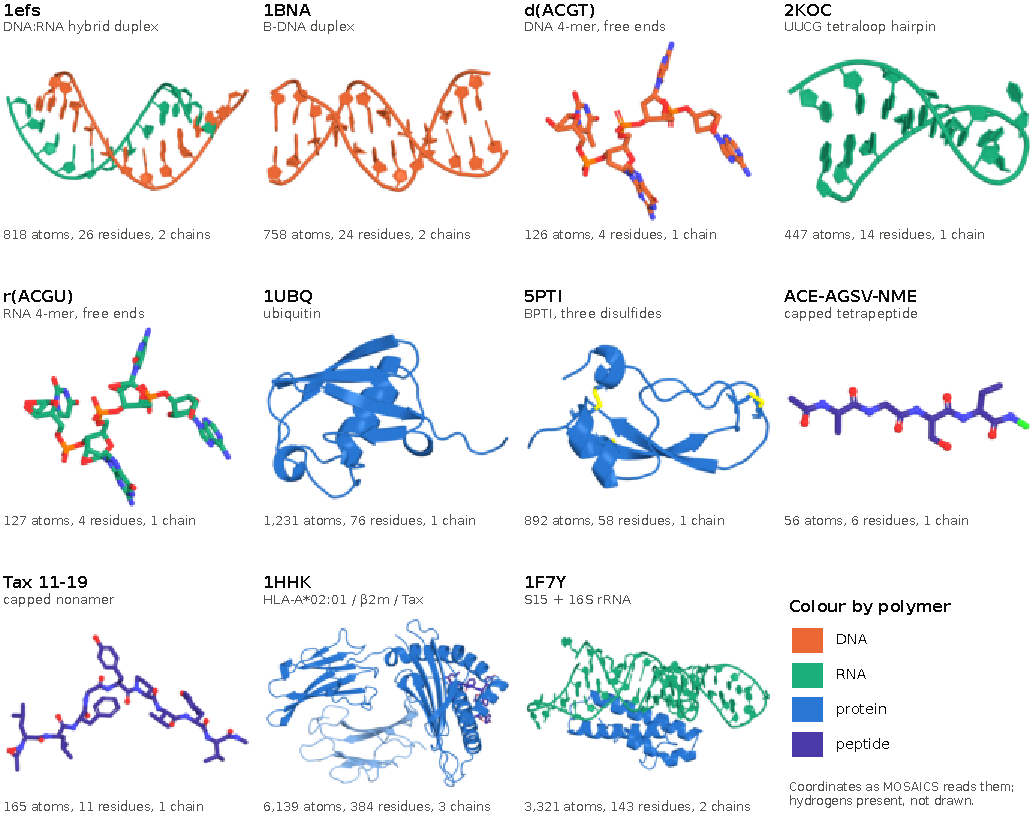
\includegraphics[width=\linewidth]{systems-gallery.pdf}
\caption{The eleven systems, drawn from the coordinates the engine reads.
Nucleic acids and proteins are shown as cartoons, the peptides and the two
free-ended 4-mers as sticks with heteroatoms coloured by element; hydrogens are
present in every file and omitted from the drawing. Chain colour follows the
polymer, with the second protein chain of 1HHK ($\beta_2$-microglobulin) in a
lighter blue and its bound Tax nonamer as violet sticks.}
\label{fig:systems}
\end{figure}

\paragraph{1efs}
A heteroduplex of one DNA strand and one RNA strand, model~1 of Protein Data
Bank entry 1EFS\cite{pdb1efs,hantz2001hybrid}. Chain A is
\texttt{DG DA DG DA DG DG DA DA DG DA DG DA DA}, six DG at 33 atoms each and
seven DA at 32, giving 422 atoms; chain B is
\texttt{RU RU RC RU RC RU RU RC RC RU RC RU RC}, seven RU at 30 atoms and six
RC at 31, giving 396. Each residue carries a charge of $-1$, so the net charge
is $-26$ and the run uses \verb|\neutralize{off}|. It is the only structure
here that mixes DNA and RNA in one duplex, and that is why it carries the
term-by-term comparison: a parameter set correct for DNA and wrong for RNA is
invisible on a pure duplex of either, and this is the system on which F-03
became visible. The coordinates are taken as deposited apart from six built
atoms, a $5'$ phosphate on each strand, and four renaming or renumbering edits,
all listed in Supporting Information section~S7. The hydrogens are the
deposited NMR hydrogens; none was rebuilt, and nothing was minimised. All four
AMBER presets build the same padded system of 942 atoms in 30 residues, then
trim four terminal residues to the 818 atoms compared, so every residue that
enters the term-by-term comparison is an interior one. The CHARMM36 cell on
this system is a different molecule: the distributed XML has no patch that both
keeps a $5'$ phosphate and ends a chain (F-08), so the structure was rebuilt as
a $5'$-OH/$3'$-OH strand, 816 atoms, six phosphate atoms removed and four
hydroxyl hydrogens added, and its total is not comparable with the AMBER rows.

\paragraph{Capped tetrapeptide}
ACE-ALA-GLY-SER-VAL-NME, 56 atoms, with four residues of four different kinds
between the two caps. The four kinds are deliberate: each interior residue
produces one $(\phi,\psi)$ correction term, ff19SB carries a different map for
different residues, and a peptide with one interior residue would resolve its
single term through a fallback and return the same energy whether the map
selection were right or wrong. The coordinates come from \texttt{tleap} and are
not minimised: what \texttt{tleap} writes is an extended chain at
$\phi=\psi=180^{\circ}$ on every residue. Two consequences run through the
paper. The out-of-plane terms sit exactly at their minima, so both MOSAICS and
GROMACS report zero for them and the comparison on that term is vacuous
(F-11); and all four correction-map terms sit at $\phi=\psi=\pi$, the singular
point of the implemented force expression, which is why every energy comparison
passed while the analytic CMAP force was identically zero (F-21).

\paragraph{The free-ended 4-mers}
d(ACGT), 126 atoms, and r(ACGU), 127 atoms, one of each base with free $5'$-OH
and $3'$-OH ends. They isolate the terminal residues, which is where the residue
templates of two force fields differ, and they carry the force sweeps, the
CHARMM36 comparison and, through the terminal decks, AMBER comparisons against
sander and OpenMM. d(ACGT) carries a geometric defect at residue DG~3, finding
F-17, set out with its consequences in Section~\ref{sec:limits}.

\paragraph{The deposited structures}
1BNA, 1UBQ, 5PTI and 2KOC were fetched from the RCSB on 25 August 2026 and
prepared under one set of rules, recorded in
\texttt{evidence-v2/\_structures/BUILD-DECISIONS.md}. Only \texttt{ATOM}
records survive; every water, ion and ligand is dropped. Alternate location A
is kept. Every hydrogen and deuterium in the deposit is stripped and rebuilt by
the topology builder, so hydrogen placement is \texttt{tleap}'s for the AMBER
decks and the OpenMM template's for the CHARMM path, never the depositor's.
Protein termini are charged, NH$_3^+$ and COO$^-$, because a whole protein is
not a fragment; nucleic termini are $5'$-OH and $3'$-OH. 1BNA is the
Drew--Dickerson dodecamer d(CGCGAATTCGCG)\cite{pdb1bna}, both strands kept
because the duplex is self-complementary and one strand is not the dodecamer,
758 atoms, net charge $-22$; its terminal residues build as DC5 and DG3. 2KOC
is model~1 of the 20-model NMR ensemble of the 14-mer cUUCGg tetraloop
hairpin\cite{pdb2koc}, GGCACUUCGGUGCC, 447 atoms; its deposited $5'$-terminal
phosphate is removed so that the chain starts at a $5'$-OH, because a bare
$5'$ phosphate is the one terminus the CHARMM36 XML cannot end a chain on, and
keeping it would have bought a second system CHARMM36 cannot run. 1UBQ is
ubiquitin\cite{pdb1ubq}, chain A, 76 residues, 1,231 atoms, net charge 0; its
one histidine, HIS~68, is built as HIE, and the C-terminal tail deposited at
occupancy 0.25--0.45 is taken as deposited. 5PTI is bovine pancreatic trypsin
inhibitor from the joint X-ray and neutron refinement\cite{pdb5pti}, chain A,
58 residues, 892 atoms, net charge $+6$; its three disulfides, CYS~5--55,
14--38 and 30--51, are built as CYX and bonded in \texttt{tleap} exactly as the
deposited SSBOND records give them, and the 103 deuterium positions of the
neutron model are stripped with the hydrogens.

\paragraph{The peptide and the two complexes}
The Tax nonamer LLFGYPVYV, the HTLV-1 epitope presented by HLA-A*02:01, is
taken from the engine's own example of that peptide, capped with ACE and NME,
165 atoms, at the main-branch commit the run record names. 1HHK is the crystal
structure of HLA-A*02:01 with $\beta_2$-microglobulin and that
nonamer\cite{pdb1hhk}, three chains of 275, 100 and 9 residues, built with
\texttt{tleap} under ff14SB and ff19SB from the prepared coordinates, 6,139
atoms with 2,978 hydrogens added, net charge $-9$. 1F7Y is ribosomal protein
S15 bound to a fragment of 16S rRNA\cite{pdb1f7y}, chain A an 86-residue
protein with charged termini and chain B a 57-nucleotide RNA, 3,321 atoms, net
charge $-49$. It is the first system run against a deck that holds protein and
RNA atom types together, and those two decks live on an engine branch that has
not been merged, which Table~\ref{tab:matrix} records. Its reference
coordinates were written from the three-decimal PDB the engine reads rather
than from \texttt{tleap}'s restart file, because the restart differs from the
PDB by up to $5\times10^{-4}$~\AA{}, which is worth 0.66~\kcal{} of
Lennard-Jones energy on this system.

One rule governs every build. \emph{The structure MOSAICS reads is the
structure the reference topology is built from, never the reverse.} MOSAICS
reads the PDB and the reference engines read the topology, and the two formats
store positions to different numbers of decimals; the largest resulting
difference on the heteroduplex was 0.0005~\AA{}. On the peptide that moved the
short-range energy by 0.573~\kcal{}, because that term rises as the twelfth
power of distance, and it looked exactly like a broken force field (F-02). The
builders write the reference positions from the structure MOSAICS reads and
refuse to continue if the two disagree.

\subsection{Run conditions}
\label{sec:methods-conditions}

Every single-point run is in vacuum, at dielectric 1, with no cutoff, no
temperature coupling, no solvent and no move. No temperature enters any number
reported in Sections~\ref{sec:coverage} to~\ref{sec:forces}: nothing is
propagated, and the one proposal that is made reproduces the current structure,
so the energy difference it is judged on is zero. A comparison counts only if
the structure did not move, and the runs check that. MOSAICS prints each part
of a term next to that term's total, so the parts must add up. On 1efs with
OL21/OL3 they do so to within $5.5\times10^{-11}$~\kcal{}, the summation order
of a double-precision sum over 818 atoms; a larger discrepancy means the
structure moved.

\subsection{The electrostatic constant}
\label{sec:methods-coulomb}

The four programs do not share the constant that converts charge into energy,
and on 1efs the disagreement is worth more than everything else being measured.
It was measured, not looked up. One AMBER topology holding two point charges,
$+1\,e$ and $-1\,e$, exactly $1.0000000000$\,\AA{} apart, with Lennard-Jones
zeroed, in vacuum and with no cutoff, is handed to every engine; the
electrostatic energy an engine then prints \emph{is} its constant. The script
is \texttt{measure\_coulomb\_constant.py} in
\texttt{evidence/coulomb-constants/}, and the four values it returns are in
Table~\ref{tab:coulomb}. sander's is measured to four digits because it prints
four decimals; its exact value is $18.2223^2 = 332.052217$, because AMBER
stores topology charges pre-multiplied by 18.2223. MOSAICS's row is analytic
rather than measured: it is the product of two constants compiled into the
engine, $0.529177\times627.50921 = 332.06344122017$, and that unrounded product
is the number every correction is done with.

Before any comparison, the electrostatic term of the MOSAICS and sander columns
is scaled by the ratio of its own constant to a single target. That target is
not any engine's measured value but a number derived from the 2019 SI values of
$e$ and $N_{\mathrm{A}}$, the thermochemical calorie and the CODATA 2018
$\varepsilon_{0}$, given in Section~\ref{sec:constant}: $k = 332.0637133$
kcal\,\AA\,mol$^{-1}$\,$e^{-2}$. The OpenMM and GROMACS columns are left as
printed: both print six decimals and to those six decimals both equal the
derived target. Every total in the 26-cell matrix and every electrostatic
residual in the term-by-term tables is on this constant.

\subsection{Force validation}
\label{sec:methods-forces}

The analytic force is compared with a central difference of the same energy,
atom by atom and component by component, for each term separately and for the
total. The step is swept over ten values from $10^{-2}$ to
$3\times10^{-7}$\,Bohr, and what is recorded at each step is the largest
$|$numerical $-$ analytic$|$ over every atom and component, in Hartree per
Bohr. Sixty-one such sweeps are committed in \texttt{evidence/forces/}:
thirty-seven against Cartesian coordinates on 1efs, the two 4-mers and the
peptide, and twenty-four against a staging coordinate, the fourth staging
system being a capped peptide fixture whose NME cap is not a physical amide and
whose energy is therefore recorded, not validated (F-18).

The measurement is the slope, not the residual. A central difference is wrong
at order step$^2$, so a force that is the derivative of the energy makes the
residual fall as the square of the step until round-off in the energy takes
over, while a force wrong by a fixed amount stops falling at that amount. The
slope is fitted by least squares on $\log_{10}$(residual) against
$\log_{10}$(step) over a window declared in advance, $10^{-2}$ to
$3\times10^{-4}$\,Bohr, four of the ten steps and spanned by every sweep.
Fixing the window matters, because a fit over rows selected for already
falling as the square would test nothing.

\subsection{The cost of one Monte Carlo step}
\label{sec:methods-cost}

A single run is setup, parse, one initial energy, $N$ steps and output. At
$N=1$ the constant part is 99.8\,\% of the wall clock, so timing one run and
calling it the cost of one evaluation would overstate it by more than two
orders of magnitude. The constant was measured instead of assumed. The
committed 1efs OL21/OL3 input was run unmodified except for
\verb|\total_step_mc| at $N = 0, 1, 5, 10, 25, 50$ and $100$, five repeats
each, and $t(N) = a + bN$ was fitted by least squares on the medians; $b$ is
the marginal cost of a step and $a$ is everything that happens once. Medians
rather than means because this is a laptop: the $N=0$ point has one 866~ms
outlier against a 442~ms floor. The build was the serial target at commit
\texttt{eccdf74}, Apple clang 21.0.0 at \texttt{-O3}, one process on one core
of an Apple M5, and the timed run is the committed run: its initial total
energy, 2526.184857387672~\kcal{}, is byte-identical to the committed
single-point output. Acceptance over the timed steps was 59 of 100. A rejected
step still costs a full energy evaluation, since the evaluation is what decides
it, so the slope is an average over a stable accept/reject mix and not a cost
conditional on acceptance.

\subsection{\studio{}}
\label{sec:methods-studio}

\studio{} is a web page. Behind it is a Python package (Python 3.10 or later,
MIT licence) whose pipeline is headless: four functions carry every operation,
\path{sequence_to_structure}, \path{structure_to_minimised},
\path{build_variant} and \path{compare_structures}, and the page calls those
functions through Pyodide. The engine is the MOSAICS executable compiled
to WebAssembly and driven through a small JavaScript bridge: the pipeline
writes the input file, the residue topology, the deck and the structure into a
run folder on the in-tab file system, runs the engine on it, follows its
progress from the lines it prints and reads back every file it writes.

\paragraph{The guided workflow}
The page presents four steps over that pipeline. \emph{Start} takes a sequence (DNA, RNA or a peptide, a pasted or
dropped FASTA record) or a coordinate file, and builds nucleic acids on ideal
A- or B-form geometry as single strands, duplexes or DNA$\cdot$RNA hybrids;
peptides are built on an ideal backbone with side chains and pH-7 protonation
from PDB2PQR's residue definitions\cite{dolinsky2004pdb2pqr,jurrus2018apbs}
and optional ACE/NME caps; proteins are prepared from coordinates, not built.
\emph{Prepare} chooses the chains to keep, leaves ligands and waters out, adds
hydrogens to a deposited protein, and chooses the force field from every
compatible profile with the reason the default was chosen; thirteen profiles
are declared, twelve over the AMBER and CHARMM36 decks of
Section~\ref{sec:methods-parameters} and one knowledge-based three-point
protein model, and each names its six files. One validation gate
sits on this step: whether the ordinary bonded and non-bonded energies for
every residue type present reproduce a committed reference. \emph{Run} offers
fifteen protocols, each with the deck it comes from, the work it is cited to
and a link to the engine's manual, and exposes every parameter the engine reads
for that kind of calculation, grouped as the manual groups them; the deck the
engine will read is one click away. \emph{Understand} shows the energy along
the run, the RMSD to the starting structure along the trajectory, energy
against RMSD with one point per frame, acceptance tallies, the energy table, a
residue-by-residue comparison of before and after, the molecular graph export
(NumPy, JSON, PyTorch Geometric and DGL formats
\cite{fey2019pyg,wang2019dgl}, with no learned embeddings), and the record.
The three-dimensional view is 3Dmol.js\cite{rego2015threedmol}, and a viewer
plays the trajectory frame by frame.

\paragraph{The record}
Every run writes a record naming the Studio version, the engine, the SHA-256 of
the engine executable, the SHA-256 of each force-field file that was staged,
the preset and every parameter it resolved, the inputs and the outputs by
digest, and the start and end times. The record and every file it names
can be downloaded from the page, and the package's verify routine recomputes
every digest and reports whether the recorded files are present and unchanged.
The engine itself already writes every parameter it resolved to
\texttt{sim\_param.out}; what the record adds is the binding of those
parameters to the engine build, the deck files and the inputs in one document
that can be re-checked.

\paragraph{The engine in the browser}
The engine was compiled to WebAssembly with Emscripten
6.0.9\cite{zakai2011emscripten} from the serial target of the engine's main
branch at commit \texttt{73f598a} (7 September 2026). The 151 objects compile
with no source changes; the link needs a 32~MB stack, because the input parser
overruns Emscripten's 64~KB default at once, and one guard on the single
\texttt{popen("date")} call, made in the scratch copy used for the build and
not in the engine repository. The result, \texttt{mosaics.wasm}, is 713,184
bytes. The Studio's own pipeline runs beside it under Pyodide
0.27.7\cite{pyodide-software} in a Web Worker; one Python shim registers the
WebAssembly build as the engine and replaces the one function that would have
launched a native executable, and everything else is the package's own code. The
distribution is about 8.5~MB of static files (the page, the engine, the Python
archive, one archive per force-field profile fetched only when that profile is
chosen, the manuals and a version manifest); a first visit downloads about
25~MB including Pyodide and NumPy from a content delivery network, cached
afterwards. Every URL the page fetches carries the build identifier, so a
redeploy is never served from a browser's cache. Nothing is uploaded and no
server computes: any static host serves it, and the copy reported here is on a
personal web page at the University of Oxford. The engine is single-threaded
in the browser, a run cannot be interrupted from outside, and everything lives
in the tab's memory until it is downloaded.

\paragraph{Tests}
The package carries 84 test files with 2,198 test functions (counted on 8
September 2026), run on every push on three operating systems across Python
3.10 to 3.13, and the browser build is checked end to end by a headless test
that drives the whole pipeline under Node with the same Python archive and the
same bridge the page uses, and fails unless the documented case study
reproduces (Section~\ref{sec:studio-results}).

\section{Results}
\label{sec:results}

\subsection{What was implemented and what was tested}
\label{sec:coverage}

Eight parameter families were converted into MOSAICS decks and evaluated at
all-atom resolution: ff14SB \cite{maier2015ff14sb} and ff19SB
\cite{tian2020ff19sb} for protein; parmbsc0 \cite{perez2007bsc0}, parmbsc1
\cite{ivani2016bsc1}, OL15/OL3 \cite{zgarbova2015ol15,zgarbova2011ol3},
OL21/OL3 \cite{zgarbova2021ol21,zgarbova2011ol3} and OL24/OL3
\cite{zgarbova2025ol24,zgarbova2011ol3} for nucleic acid; and CHARMM36 for
nucleic acid \cite{hart2012charmm36dna,denning2011charmm36rna}. Across the
eleven systems they give the 26 system-and-force-field combinations of
Table~\ref{tab:matrix}, 54 MOSAICS-to-reference comparisons in all, 20 of the
26 cells carrying two or more references.

The cells were not all checked to the same strength, and the table says which
is which. The six original AMBER combinations on the heteroduplex and the
tetrapeptide were compared term by term against all three references, and the
ff14SB proteins and the OL21/OL3, OL15/OL3 and OL3 nucleic systems have a
GROMACS total as well as sander and OpenMM. Every ff19SB row is against sander
and OpenMM only, because the ParmEd route collapses its per-residue correction
maps onto one (F-06, Section~\ref{sec:methods-references}); the GROMACS cell is
blank, not failing. The CHARMM36 and OL24 rows are against OpenMM only.
CHARMM36 has one reference because its deck and its reference are both read
out of the same OpenMM build; on the Drew--Dickerson dodecamer the sander OL24
run read the full-precision restart coordinates where MOSAICS and OpenMM read
the three-decimal PDB, so it is a comparison of two geometries and is left out.
The 1efs CHARMM36 cell is the 816-atom $5'$-OH rebuild of the heteroduplex
(F-08) and is not comparable with the AMBER rows above it. The two 1F7Y rows
run on decks that exist only on an unmerged engine branch. Every run is a
single-point energy at one fixed geometry, in vacuum, with no cutoff and
dielectric~1.

\paragraph{Which chemistry the test systems reach}
A deck is a table, and a single-point energy exercises only the rows the
structure selects. The eleven systems reach all eight standard nucleic bases,
DA, DC, DG and DT on the dodecamer and A, C, G and U on the tetraloop and the
RNA 4-mer; $5'$-OH and $3'$-OH chain ends on five systems and $5'$-phosphate
interior chemistry on the padded heteroduplex; twenty amino-acid types across
ubiquitin, BPTI and the MHC heavy chain, including charged, aromatic,
histidine and proline residues, three disulfides, charged termini and two
capped fragments. What no system reaches is a $5'$-phosphate terminus under
any deck, an alternative protonation state, or more than one conformation: each
cell is one geometry, so a parameter that is wrong but inactive at that
geometry, or a torsion whose phase is wrong but degenerate there, would not
show. Finding F-21 is that failure mode caught in the act: an analytic force
that was identically zero passed every energy comparison on the peptide.

\subsection{Single-point agreement over 26 combinations}
\label{sec:matrix}

Table~\ref{tab:matrix} gives every total energy as each program returns it,
with the electrostatic term of MOSAICS and sander rescaled to the single
constant of Section~\ref{sec:constant}, and the difference of each reference
from MOSAICS. Figure~\ref{fig:energy-agreement} plots the same 54 differences,
and, where the engine output files resolve them, the differences term by term.

\begin{table}[tbp]
\centering
\footnotesize
\setlength{\tabcolsep}{4pt}
\caption{Single-point total energies on the eleven systems, in \kcal{}, vacuum,
no cutoff, every electrostatic term on the CODATA-derived constant
$332.0637133$. A dash means that reference was not run for that cell, for the
reason given in Section~\ref{sec:coverage}. The right-hand block is the
reference minus MOSAICS. The 1efs CHARMM36 row is the 816-atom $5'$-OH
rebuild of the heteroduplex, not the 818-atom structure of the rows above it;
the 1F7Y decks are on an unmerged engine branch. Source:
\texttt{work/preprint-I/energies/MATRIX.json}, and the engine output files it
names; the table is written from that file by \texttt{make\_tables.py}.}
\label{tab:matrix}
\resizebox{\textwidth}{!}{% generated by make_tables.py from energies/MATRIX.json
\begin{tabular}{@{}llrrrrrrr@{}}
\toprule
 & & \multicolumn{4}{c}{Total energy (kcal/mol)} & \multicolumn{3}{c}{Reference minus MOSAICS (kcal/mol)} \\
\cmidrule(lr){3-6}\cmidrule(lr){7-9}
System & Force field & MOSAICS & sander & OpenMM & GROMACS & sander & OpenMM & GROMACS \\
\midrule
1efs & OL21/OL3 & 2526.186378 & 2526.186713 & 2526.186575 & 2526.186580 & +0.000335 & +0.000197 & +0.000202 \\
 & OL15/OL3 & 2522.856302 & 2522.856613 & 2522.856501 & 2522.856506 & +0.000311 & +0.000199 & +0.000204 \\
 & OL24/OL3 & 2954.803590 & -- & 2954.803568 & -- & -- & -0.000022 & -- \\
 & CHARMM36 & 3775.995925 & -- & 3775.995927 & -- & -- & +0.000002 & -- \\
1BNA & OL21 & 2141.488688 & 2141.487481 & 2141.487431 & 2141.488017 & -0.001208 & -0.001258 & -0.000671 \\
 & OL15 & 2138.533139 & 2138.531881 & 2138.531881 & 2138.532468 & -0.001258 & -0.001258 & -0.000671 \\
 & CHARMM36 & 3509.022307 & -- & 3509.022309 & -- & -- & +0.000001 & -- \\
 & OL24 & 2954.122454 & -- & 2954.122861 & -- & -- & +0.000407 & -- \\
d(ACGT) & OL21 & 942.827346 & 942.827874 & 942.827764 & -- & +0.000528 & +0.000418 & -- \\
 & OL15 & 945.670885 & 945.671374 & 945.671303 & -- & +0.000489 & +0.000418 & -- \\
 & OL24 & 1080.088750 & -- & 1080.088749 & -- & -- & -0.000000 & -- \\
2KOC & OL3 & 347.450922 & 347.450964 & 347.451027 & 347.450987 & +0.000042 & +0.000106 & +0.000065 \\
 & CHARMM36 & 2106.624466 & -- & 2106.624466 & -- & -- & +0.000000 & -- \\
r(ACGU) & OL3 & 2584.335888 & 2584.336025 & 2584.335946 & -- & +0.000137 & +0.000058 & -- \\
1UBQ & ff14SB & -546.960403 & -546.959674 & -546.959594 & -546.959625 & +0.000729 & +0.000809 & +0.000778 \\
 & ff19SB & -1022.050252 & -1022.050874 & -1022.050802 & -- & -0.000622 & -0.000550 & -- \\
5PTI & ff14SB & -332.312157 & -332.311788 & -332.311563 & -332.311590 & +0.000369 & +0.000594 & +0.000567 \\
 & ff19SB & -688.753926 & -688.711488 & -688.711342 & -- & +0.042438 & +0.042584 & -- \\
ACE-AGSV-NME & ff14SB & 96.262476 & 96.262430 & 96.262484 & 96.262481 & -0.000046 & +0.000008 & +0.000005 \\
 & ff19SB & 69.244797 & 69.244830 & 69.244805 & -- & +0.000033 & +0.000008 & -- \\
Tax 11--19 & ff14SB & -23.358508 & -23.358422 & -23.358416 & -- & +0.000087 & +0.000092 & -- \\
 & ff19SB & -82.278687 & -82.278622 & -82.278606 & -- & +0.000066 & +0.000081 & -- \\
1HHK & ff14SB & -475.878441 & -475.874656 & -475.873684 & -- & +0.003785 & +0.004757 & -- \\
 & ff19SB & -2937.222999 & -2937.219256 & -2937.218706 & -- & +0.003743 & +0.004293 & -- \\
1F7Y & ff14SB/OL3 & 14238.328640 & 14238.329782 & 14238.329881 & -- & +0.001142 & +0.001241 & -- \\
 & ff19SB/OL3 & 13685.351529 & 13685.353082 & 13685.353068 & -- & +0.001553 & +0.001539 & -- \\
\bottomrule
\end{tabular}
}
\end{table}

\begin{figure}[tbp]
\centering
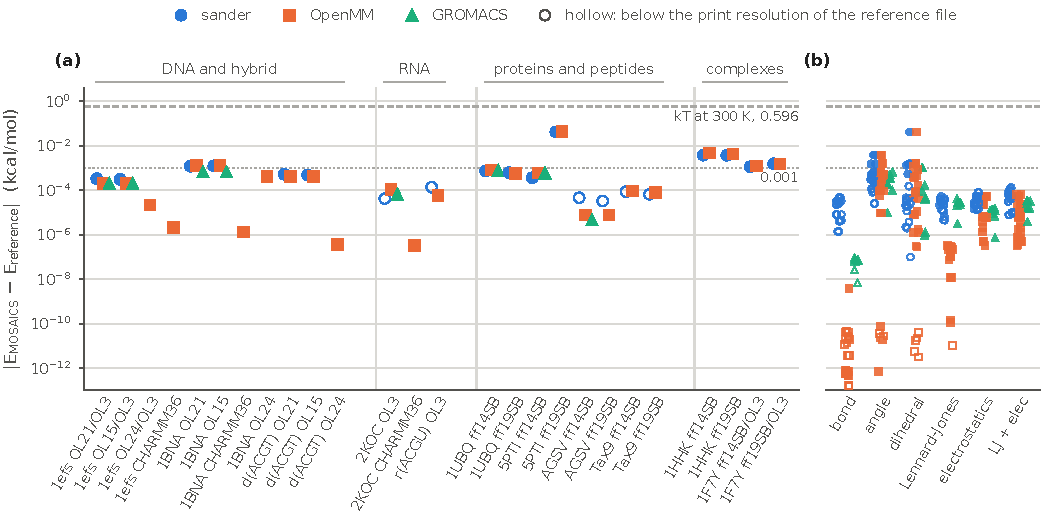
\includegraphics[width=\linewidth]{energy-agreement.pdf}
\caption{Energy agreement over the 26 combinations. (a) One marker per
MOSAICS-to-reference comparison of the total energy, 54 in all, grouped by
system class; the vertical axis is $|E_{\mathrm{MOSAICS}} -
E_{\mathrm{reference}}|$ on a log scale. Marker shape and colour identify the
reference engine. (b) The same comparisons resolved into the terms the engines
share, for the cells whose output files carry the split; where an OpenMM file
prints only a combined non-bonded energy the comparison appears in the last
column. Hollow markers fall below the print resolution of the reference file
they were read from and are print quantisation, not measured disagreement.
Dashed line, $kT$ at 300~K, 0.596~\kcal{}; dotted line, 0.001~\kcal{}. Every
value is re-derived from \texttt{MATRIX.json} and the engine outputs it names
by \texttt{figures/energy-agreement.py}.}
\label{fig:energy-agreement}
\end{figure}

Nineteen of the 26 cells agree with every reference available to them to
within 0.001~\kcal{}, and thirteen to within 0.0004. Over the 26 cells the
median of the largest gap to any reference is 0.00037~\kcal{}; the smallest is
$3.2\times10^{-7}$, on the tetraloop under CHARMM36, and the largest is
0.0426, on BPTI under ff19SB. For scale, $kT$ at 300~K is 0.596~\kcal{}, and the
sander column can resolve nothing below about $2\times10^{-4}$. The seven cells
outside 0.001~\kcal{} are, in order, BPTI ff19SB (0.0426), the two
peptide--MHC cells (0.0048 and 0.0043), the two S15--rRNA cells (0.0012 and
0.0016) and the dodecamer under OL21 and OL15 (0.0013 each). Each has a
mechanism, and they are of three kinds.

\paragraph{An improper read in two atom orders}
The BPTI ff19SB cell is 0.0426~\kcal{} below the references on the dihedral
term and nowhere else: bond, angle, Lennard-Jones and electrostatics carry the
same residuals as the ff14SB cell on the same coordinates, and the correction
map matches OpenMM to $5.8\times10^{-13}$. Splitting the dihedral term puts
the whole gap in the impropers, 5.5085 against 5.5506~\kcal{}. It is one
improper, at the backbone nitrogen of ASP~3. The AMBER topology writes that
improper in the order C--CA--N--H and the MOSAICS residue template in the order
$-$C--H--N--CA; the two orders define different dihedral angles, which coincide
when the nitrogen is planar and part company when it is not, and at ASP~3 in
the deposited coordinates they read $-156.8^{\circ}$ and $+158.4^{\circ}$,
some $22^{\circ}$ from planar. Evaluating that one improper in the topology's
order, with the two conventions for the phase and the deck's coefficient
rounding accounted for, reproduces the whole gap to $8.5\times10^{-8}$~\kcal{},
and the accounting is committed beside the run. The same mechanism produced a
0.46~\kcal{} gap at LEU~2 of the Tax nonamer on an earlier build of that
structure, which is why the peptide's first amide hydrogen is now placed in the
peptide plane by the engine's builder and why the nonamer cells in
Table~\ref{tab:matrix} agree to $9\times10^{-5}$. The ff14SB cell on the same
BPTI coordinates is within $6\times10^{-4}$, so the parameters are not in
question: the improper order is.

\paragraph{Six adenine impropers on the dodecamer}
Under OL21 and OL15 the dodecamer sits 0.0013~\kcal{} above sander and OpenMM
and 0.0007 above GROMACS. Resolved into terms the excess is on the torsion
term, $+1.5\times10^{-3}$, of which $+1.0\times10^{-3}$ is improper, and it
was located rather than guessed. \texttt{tleap} under DNA.OL21 writes the
adenine N9 improper as C8/C4/N9/C1$'$ and under ff99bsc0 as C4/C8/N9/C1$'$;
swapping the first two atoms is not a symmetry of the term when the group is
not exactly planar; MOSAICS agrees with the parmbsc0 order to eight figures,
and the six instances that differ, on DA~5, 16 and 17, account for the whole
$1.0\times10^{-3}$. The same term on the heteroduplex, whose entire improper
energy is $5.3\times10^{-4}$~\kcal{}, is within $4.3\times10^{-5}$, so the
difference between the two structures is the geometry the impropers are
evaluated at, not the parameters.

\paragraph{Two large systems not yet resolved into terms}
The peptide--MHC complex, 6,139 atoms, is 0.0038~\kcal{} above sander and 0.0048
above OpenMM under ff14SB, and 0.0037 and 0.0043 under ff19SB, out of a total of
$-476$ and $-2937$; per atom that is below $10^{-6}$~\kcal{}, and the two
force fields give the same offset within $5\times10^{-4}$, which points at the
non-bonded or angle terms they share rather than at the backbone terms they do
not. The S15--rRNA complex, 3,321 atoms, is 0.0012 and 0.0016~\kcal{} below the
references, and its terms are resolved: bond agrees to $2\times10^{-11}$, the
correction map to $2\times10^{-11}$, torsion and improper to $4\times10^{-4}$
and $8\times10^{-5}$, while the angle term carries $-1.55\times10^{-3}$ and the
non-bonded sum $-3.7\times10^{-3}$ in the two directions that nearly cancel.
Those two systems are the only ones whose reference coordinates were written
from the three-decimal PDB rather than from \texttt{tleap}'s restart, and the
S15--rRNA decks are on a branch; both cells are reported as they stand and
neither is claimed to be closed.

\paragraph{The angle term, on every system}
The one residual that appears on every system whose terms were resolved is on
the angle term, and it always has the same sign. MOSAICS minus OpenMM on that
term is $-1.76\times10^{-4}$~\kcal{} on the heteroduplex, $-9.6\times10^{-6}$
on the tetrapeptide, $-1.0\times10^{-4}$ on the tetraloop, $-3.4\times10^{-4}$
on the dodecamer, $-5.1\times10^{-4}$ on BPTI and $-6.5\times10^{-4}$ on
ubiquitin, growing with the number of angles. It is not a MOSAICS error. The
AMBER topology builder writes every equilibrium angle as the published value
multiplied by a seven-digit approximation of $\pi/180$, while MOSAICS reads the
value in degrees and converts it exactly, so the reference carries the rounding
(F-12). It is reported and not corrected, and it is the largest residual on
every AMBER cell that is inside 0.001~\kcal{}.

\subsection{Term by term on the two reference systems}
\label{sec:energies}

Before the numbers, the resolution of the files they are read from, because
several of the differences below are smaller than the output they come out of.
sander prints four decimals, an absolute floor near $2\times10^{-4}$~\kcal{}.
GROMACS energies are read from \texttt{sp.xvg}, which carries six decimals in
kJ/mol, a floor of $2.4\times10^{-7}$~\kcal{}. OpenMM's single-point output
carries twelve decimal places, a floor of about $5\times10^{-13}$~\kcal{}.
MOSAICS prints sixteen significant digits. A difference smaller than the floor
of the file it is taken from is the last printed digit of that file and not a
measurement, and no such number is quoted here as a residual.

On every one of the six original AMBER combinations, the largest difference
between MOSAICS and OpenMM on any energy term is $1.8\times10^{-4}$~\kcal{} for
the four heteroduplex decks and $9.6\times10^{-6}$~\kcal{} for the two peptide
decks, in both cases on the angle term and for the reason just given. Every
other term on every other row is smaller than this. The margin varies widely:
the parmbsc1 dihedral residual, $+1.03\times10^{-4}$~\kcal{}, is within a factor
of two of it, while the two peptide bond terms agree past the twelfth decimal
place OpenMM writes, which is as far as the comparison can be taken and no
further. Table~\ref{tab:ol21} gives the full four-engine breakdown for one force
field, OL21/OL3 on 1efs, so that the raw numbers are on the page, and
Table~\ref{tab:summary} gives MOSAICS minus each reference, per term, for all
six combinations.

\begin{table}[t]
\centering
\small
\setlength{\tabcolsep}{5pt}
\caption{OL21/OL3 on 1efs (818 atoms, net charge $-26$, vacuum, no cutoff), in
\kcal{}, as each engine prints them. The dihedral row includes impropers, and the
Lennard-Jones and electrostatic rows include the 1--4 terms. sander gives four
decimals (floor $2\times10^{-4}$~\kcal{}), the GROMACS column is converted from
\texttt{sp.xvg} values carrying six decimals in kJ/mol (floor
$2.4\times10^{-7}$), OpenMM writes twelve decimals (floor $5\times10^{-13}$)
and MOSAICS writes sixteen significant digits. \emph{corrected} means the
electrostatic term rescaled to the single constant of
Section~\ref{sec:constant}; the MOSAICS column is divided by the unrounded
product $0.529177\times627.50921$ and the sander column by
$18.2223^{2}=332.05221729$, so either corrected entry can be reproduced digit
for digit from the printed one above it. Sources:
\texttt{evidence/1efs/ol21\_ol3/\{mosaics,sander,openmm,gromacs\}/}.}
\label{tab:ol21}
\begin{tabular}{@{}lrrrr@{}}
\toprule
Term & MOSAICS & sander & OpenMM & GROMACS \\
\midrule
bond                   &   70.99877741 &   70.9988    &   70.99877741 &   70.99877749 \\
angle                  &  220.56489609 &  220.5651    &  220.56507252 &  220.56507290 \\
dihedral               &  596.17955421 &  596.1796    &  596.17959679 &  596.17959369 \\
Lennard-Jones          & $-$219.29643681 & $-$219.2964 & $-$219.29643710 & $-$219.29646343 \\
electrostatic, printed & 1857.73806648 & 1857.6753    & 1857.73956494 & 1857.73959895 \\
electrostatic, corrected & 1857.73958864 & 1857.73961475 & 1857.73956494 & 1857.73959895 \\
\midrule
total, corrected       & 2526.18637954 & 2526.18671475 & 2526.18657455 & 2526.18657959 \\
\bottomrule
\end{tabular}
\end{table}

\begin{table}[t]
\centering
\footnotesize
\setlength{\tabcolsep}{2.5pt}
\caption{MOSAICS minus each reference engine, per term, in \kcal{}, on the six
original combinations. Electrostatics are corrected on both sides to
$332.0637133$~kcal\,\AA\,mol$^{-1}$\,$e^{-2}$ (Section~\ref{sec:constant})
before the difference is taken, with the MOSAICS side divided by the unrounded
$0.529177\times627.50921 = 332.06344122017$. \emph{n.r.} means the difference
is smaller than the resolution of that reference's own output file, so the
value in the committed evidence is a print artefact; the 27 censored sander
entries run from $2.0\times10^{-6}$ to $5.1\times10^{-5}$ in the raw files.
The GROMACS CMAP entry is the conversion-route limit F-06 and not a
disagreement about physics. \emph{--} marks a term the force field does not
have. Source: \texttt{evidence/results.txt} and the per-combination output
files under \texttt{evidence/}.}
\label{tab:summary}
\begin{tabular}{@{}lrrrrrr@{}}
\toprule
Term & OL21/OL3 & OL15/OL3 & parmbsc1 & parmbsc0 & ff14SB & ff19SB \\
\midrule
\multicolumn{7}{@{}l}{\emph{Reference: OpenMM 8.5.2, output floor $5\times10^{-13}$~\kcal{}}}\\
bond      & n.r. & $+3.78\times10^{-9}$ & $-8.30\times10^{-8}$ & $-8.30\times10^{-8}$ & n.r. & n.r. \\
angle     & $-1.76\times10^{-4}$ & $-1.76\times10^{-4}$ & $-1.76\times10^{-4}$ & $-1.76\times10^{-4}$ & $-9.57\times10^{-6}$ & $-9.57\times10^{-6}$ \\
dihedral  & $-4.26\times10^{-5}$ & $-4.45\times10^{-5}$ & $+1.03\times10^{-4}$ & $+3.59\times10^{-5}$ & $+1.27\times10^{-6}$ & $+1.28\times10^{-6}$ \\
cmap      & --  & --  & --  & --  & --  & $-5.69\times10^{-8}$ \\
Lennard-Jones & $+2.89\times10^{-7}$ & $+2.71\times10^{-7}$ & $+3.81\times10^{-6}$ & $+3.81\times10^{-6}$ & $+1.15\times10^{-8}$ & $+1.15\times10^{-8}$ \\
electrostatic & $+2.37\times10^{-5}$ & $+2.37\times10^{-5}$ & $+2.37\times10^{-5}$ & $+2.37\times10^{-5}$ & $+4.18\times10^{-7}$ & $+4.18\times10^{-7}$ \\
\addlinespace
\multicolumn{7}{@{}l}{\emph{Reference: sander 24.0, output floor $2\times10^{-4}$~\kcal{}}}\\
bond      & n.r. & n.r. & n.r. & n.r. & n.r. & n.r. \\
angle     & $-2.04\times10^{-4}$ & $-2.04\times10^{-4}$ & $-2.04\times10^{-4}$ & $-2.04\times10^{-4}$ & n.r. & n.r. \\
dihedral  & n.r. & n.r. & n.r. & n.r. & n.r. & n.r. \\
cmap      & --  & --  & --  & --  & --  & n.r. \\
Lennard-Jones & n.r. & n.r. & n.r. & n.r. & n.r. & n.r. \\
electrostatic & n.r. & n.r. & n.r. & n.r. & n.r. & n.r. \\
\addlinespace
\multicolumn{7}{@{}l}{\emph{Reference: GROMACS 2025.4, output floor $2.4\times10^{-7}$~\kcal{}}}\\
bond      & n.r. & n.r. & n.r. & n.r. & n.r. & n.r. \\
angle     & $-1.77\times10^{-4}$ & $-1.77\times10^{-4}$ & $-1.77\times10^{-4}$ & $-1.77\times10^{-4}$ & $-9.60\times10^{-6}$ & $-9.60\times10^{-6}$ \\
dihedral  & $-3.95\times10^{-5}$ & $-4.16\times10^{-5}$ & $+1.07\times10^{-4}$ & $+3.90\times10^{-5}$ & $+1.30\times10^{-6}$ & $+1.38\times10^{-6}$ \\
cmap      & --  & --  & --  & --  & --  & $-3.02\times10^{-1}$ (F-06) \\
Lennard-Jones & $+2.66\times10^{-5}$ & $+2.66\times10^{-5}$ & $+3.01\times10^{-5}$ & $+3.01\times10^{-5}$ & $+3.02\times10^{-6}$ & $+3.02\times10^{-6}$ \\
electrostatic & $-1.03\times10^{-5}$ & $-1.03\times10^{-5}$ & $-1.03\times10^{-5}$ & $-1.03\times10^{-5}$ & $+6.49\times10^{-7}$ & $+6.49\times10^{-7}$ \\
\bottomrule
\end{tabular}
\end{table}

\paragraph{On the two non-bonded terms, the reference engines disagree with each
other more than MOSAICS disagrees with either}
OpenMM and GROMACS are independently written codes, and on 1efs they were given
the same parameters and the same coordinates. They differ from one another by
$+2.63\times10^{-5}$~\kcal{} on Lennard-Jones and $-3.40\times10^{-5}$ on
electrostatics, on all four nucleic decks. MOSAICS minus OpenMM on the same two
terms is $+2.89\times10^{-7}$ on Lennard-Jones under OL21/OL3
($+3.81\times10^{-6}$ under the two bsc decks) and $+2.20\times10^{-5}$ on
electrostatics, the latter with both sides corrected to OpenMM's own printed
constant. That pattern, bonded terms with few parameters surviving and
non-bonded terms with thousands not, is what a text-format topology conversion
would produce, since a GROMACS \texttt{.top} stores fewer digits per parameter
than the binary topology the other two engines read. We have not tested that
attribution directly. What the numbers establish is a bound that has nothing to
do with MOSAICS: two mature MD codes, handed the same force field through the
ordinary conversion route, land $3\times10^{-5}$~\kcal{} apart on an 818-atom
system, and on the two non-bonded terms MOSAICS sits below that bound against
either reference.

\paragraph{The peptide test is a targeted test of what ff19SB adds}
Between ff14SB and ff19SB on the same capped peptide, the bond, angle,
Lennard-Jones and electrostatic terms are bit-identical in all four engines.
MOSAICS returns the same bond (0.14749181), bend (0.98732525), Lennard-Jones
(134.50567845) and electrostatic ($-71.35989834$~\kcal{}) energies in both
runs, agreeing to the last of the sixteen digits it prints. The whole ff14SB-to-ff19SB difference is
$-27.01767928$~\kcal{}, of which $-25.09643922$ is the backbone torsion and
$-1.92124006$ is the correction map; every other term contributes exactly zero.
The ff19SB row is therefore the correction-map machinery applied on top of an
already-verified ff14SB, tested with everything else held fixed, and four
residues select four of the sixteen maps the deck loads. On ubiquitin, BPTI and
the two complexes the same machinery is exercised on every amino-acid type the
deck holds, and the correction-map term matches OpenMM to between
$3\times10^{-13}$ and $2\times10^{-11}$~\kcal{} on all six ff19SB cells.

\paragraph{The nucleic decks are different parameter sets, and each is
reproduced as it stands}
All three references return the same bond, angle, Lennard-Jones and
electrostatic energies for all four AMBER nucleic decks on 1efs; only the
dihedral term moves. That is the design of those decks showing through, and it
makes the dihedral row of Table~\ref{tab:summary} the row that carries the
result: MOSAICS follows each of the four dihedral values to between
$3.6\times10^{-5}$ and $1.0\times10^{-4}$~\kcal{} against OpenMM and GROMACS,
without being retuned for any of them. On the tetraloop the OL15/OL3 and OL21/OL3
terminal decks return the same energy, 347.4514261182977~\kcal{} before the
constant correction, to all sixteen printed digits on every term, because OL15
and OL21 touch DNA torsions only and a pure RNA chain never reaches them;
Table~\ref{tab:matrix} carries that one measurement once, as OL3. The
size of the gap between two decks' absolute torsion energies is not reported
here and is not a quantity this protocol can produce.

\paragraph{CHARMM36 nucleic acid, one reference}
An OpenMM reference for the CHARMM36 nucleic deck was built from
\texttt{charmm36\_2024.xml} and evaluated on the two free-ended 4-mers, the
dodecamer, the tetraloop and the $5'$-OH rebuild of the heteroduplex. The deck
covers 24 residues (every base as a $5'$, internal and $3'$ unit, DNA and RNA)
with 237 bonds, 562 bends, 1036 torsion entries and 15\,753 non-bonded pairs.
Table~\ref{tab:charmm36} gives the two 4-mers term by term. Every bonded term
matches to the digits OpenMM prints, and that includes the two CHARMM terms the
AMBER force fields do not have, the Urey--Bradley 1--3 harmonics and the
harmonic impropers. What the improper row shows needs care: its total is
$1.0\times10^{-3}$~\kcal{} over 188 terms, so the structure sits at the improper
minimum for practical purposes, and that is exactly where the engine's truncated
sixth-order expansion and CHARMM's quadratic coincide by construction.
Ten-digit agreement there confirms that the 188 entries were converted and
selected correctly; it does not exercise the functional form away from
equilibrium. The electrostatic term is the only one that does not match as
printed, at $9.8\times10^{-5}$~\kcal{} on the RNA 4-mer and $2.9\times10^{-4}$
on the DNA 4-mer, and the charge-to-energy constant accounts for that offset to
four significant figures: corrected exactly as the AMBER rows are corrected, the
two residuals fall to $-2.4\times10^{-10}$ and $-9.0\times10^{-10}$~\kcal{}. On
the three larger structures the corrected totals differ from OpenMM by
$-3.5\times10^{-7}$ (dodecamer), $+3.2\times10^{-7}$ (tetraloop) and
$-2.1\times10^{-6}$~\kcal{} (816-atom heteroduplex). That is the closest
agreement anywhere in this work, and Section~\ref{sec:constantgeneral} says
why.

\begin{table}[t]
\centering
\small
\caption{CHARMM36 nucleic acid against OpenMM 8.5.2, in \kcal{}, on the two
free-ended 4-mers with 5TER/3TER termini in vacuum, as printed. r(ACGU) is 127
atoms and d(ACGT) is 126. Urey--Bradley is CHARMM's 1--3 harmonic term, which in
OpenMM sits inside \texttt{HarmonicBondForce} and is separated here. The two
d(ACGT) bonded columns are inflated by a defect in that committed structure, in
which one H--C--H angle is $3.15^{\circ}$ instead of $109.5^{\circ}$ (F-17,
Section~\ref{sec:limits}); the comparison between the two programs is
unaffected, because both read the same coordinates. The electrostatic rows
differ by the charge-to-energy constant and by little else. Sources:
\texttt{evidence/charmm36\_rna\_acgu.tsv}, \texttt{evidence/charmm36\_dna\_acgt.tsv}.}
\label{tab:charmm36}
\begin{tabular}{@{}lrrrr@{}}
\toprule
& \multicolumn{2}{c}{r(ACGU)} & \multicolumn{2}{c}{d(ACGT)} \\
\cmidrule(lr){2-3}\cmidrule(lr){4-5}
Term & MOSAICS & OpenMM & MOSAICS & OpenMM \\
\midrule
bond           &   28.51501806 &   28.51501806 &   18.92184909 &   18.92184909 \\
Urey--Bradley  &   27.33939420 &   27.33939420 &  167.65137978 &  167.65137978 \\
angle          &  166.36120948 &  166.36120948 &  412.78809431 &  412.78809431 \\
torsion        &  114.02952401 &  114.02952401 &  122.94661546 &  122.94661546 \\
improper       &    0.00102252 &    0.00102252 &    0.00102555 &    0.00102555 \\
1--4 Lennard-Jones & 230.89575106 & 230.89575106 & 1412.27140098 & 1412.27140098 \\
Lennard-Jones  & 2564.74970076 & 2564.74970076 &  176.68820406 &  176.68820406 \\
electrostatic  & $-$119.98431509 & $-$119.98441340 & $-$356.57731681 & $-$356.57760898 \\
\midrule
total          & 3011.90730500 & 3011.90720669 & 1954.69125242 & 1954.69096025 \\
\bottomrule
\end{tabular}
\end{table}

\subsection{The charge-to-energy constant, and why every electrostatic number is corrected}
\label{sec:constant}

The four programs do not use the same constant to turn charges into an energy.
This was measured and not assumed, by the two-charge topology of
Section~\ref{sec:methods-coulomb}, and Table~\ref{tab:coulomb} gives the four
values. Every electrostatic term in this work is put on one target constant
before any difference is taken, and that target has to be a number with a
derivation, or the correction becomes a preference. It is
\begin{equation*}
  \frac{e^2 N_{\mathrm A}}{4\pi\varepsilon_0 \times 1\,\text{\AA} \times
  4.184\,\mathrm{J\,cal^{-1}}}
  = 332.0637133\ \mathrm{kcal}\,\text{\AA}\,\mathrm{mol}^{-1}\,e^{-2},
\end{equation*}
evaluated with the CODATA 2018 recommended values\cite{codata2018}. The
elementary charge, $e = 1.602176634\times10^{-19}$~C, and the Avogadro
constant, $N_{\mathrm A} = 6.02214076\times10^{23}$~mol$^{-1}$, are both exact
by the 2019 SI definitions; $\varepsilon_0 = 8.8541878128\times10^{-12}$
F\,m$^{-1}$; and the thermochemical calorie is exactly 4.184~J. The 2022 revision of $\varepsilon_0$ gives $332.0637131$
instead, lower by $6.8\times10^{-10}$ relative, which is worth
$1.3\times10^{-6}$~\kcal{} on the 1efs electrostatic term.

\begin{table}[t]
\centering
\small
\caption{The charge-to-energy constant of each program, in
kcal\,\AA\,mol$^{-1}$\,e$^{-2}$. sander, OpenMM and GROMACS were measured with
two unit charges 1~\AA{} apart in vacuum, everything else switched off; the
MOSAICS entry is evaluated from the constants compiled into the engine,
$0.529177 \times 627.50921$. sander's measured value is limited by its
four-decimal print precision; its exact value is $18.2223^2 = 332.05221729$,
and that full value is what corrects the sander column. The OpenMM and GROMACS
measurements were recorded to six decimals, which bounds their relative
difference from the target at $1.5\times10^{-9}$ and says nothing finer.
Source: \texttt{evidence/coulomb-constants/}.}
\label{tab:coulomb}
\begin{tabular}{@{}lrrr@{}}
\toprule
Engine & Constant & Relative to sander & Relative to $332.0637133$ \\
\midrule
sander  & 332.052200 & $0$                   & $-3.5\times10^{-5}$ \\
OpenMM  & 332.063713 & $+3.467316\times10^{-5}$ & $<1.5\times10^{-9}$, print-limited \\
GROMACS & 332.063713 & $+3.467284\times10^{-5}$ & $<1.5\times10^{-9}$, print-limited \\
MOSAICS & 332.063441 & $+3.385377\times10^{-5}$ & $-8.2\times10^{-7}$ \\
\bottomrule
\end{tabular}
\end{table}

sander is the outlier, not MOSAICS. It stores topology charges pre-multiplied
by 18.2223 and its constant is that number squared, which is an older value;
OpenMM and GROMACS, written independently of each other, agree with each other
and with the derived target to every decimal their measurement was recorded to.
MOSAICS sits $8.2\times10^{-7}$ below the target because three constants
compiled into the engine are rounded (F-13). The size of this effect exceeds
every difference the comparison is trying to resolve. On 1efs the sander
electrostatic term moves by $+0.0643147$~\kcal{} when rescaled, and the MOSAICS
term by $+1.522158\times10^{-3}$; the sander shift is roughly 360 times the
largest residual left after correction and about a tenth of $kT$ at 300~K. An
uncorrected cross-engine comparison of an 818-atom charged system would
therefore report a disagreement between sander and OpenMM bigger than
everything else on the page, and it would be reporting a unit convention.

Which constant is the target has to be stated, because the choice is worth
something. Corrected to OpenMM's own printed constant instead of the derived
one, MOSAICS minus OpenMM on electrostatics is $+2.202\times10^{-5}$~\kcal{} on
all four 1efs rows against the $+2.370\times10^{-5}$ of
Table~\ref{tab:summary}; the $1.68\times10^{-6}$ between the two frames is what
a six-decimal printed constant costs, and neither choice changes any
conclusion. After correction, $+2.37\times10^{-5}$~\kcal{} remains on the 1efs
electrostatic term, $1.3\times10^{-8}$ of the term, and we cannot account for
it. One hypothesis fits what is on the page. The AMBER decks reach MOSAICS
through a text route, and a prmtop writes charges in \texttt{\%FORMAT(5E16.8)},
about $10^{-8}$ relative per charge, the same order as the residual; the
CHARMM36 deck does not take that route, its charges are read out of a built
OpenMM \texttt{System} at full double precision, and its corrected residuals
are three orders of magnitude smaller on the same engine with the same
correction. Testing this needs a diff of the deck charges against the prmtop
charges at full precision, which is one command and is not in the evidence.

\subsection{Forces}
\label{sec:forces}

Analytic forces were checked against a central difference of the same energy,
term by term, over a ten-point step sweep from $10^{-2}$ to $3\times10^{-7}$
Bohr, on six Cartesian systems and, against a staging coordinate, on four
staged systems: 61 sweeps in all, covering five terms and their sum on every
system, plus the correction map on the ff19SB peptide. The residual is the
largest $|$numerical $-$ analytic$|$ over every atom and every component at a
given step. Figure~\ref{fig:force-convergence} plots the total-energy sweep on
six of the systems.

\begin{figure}[tbp]
\centering
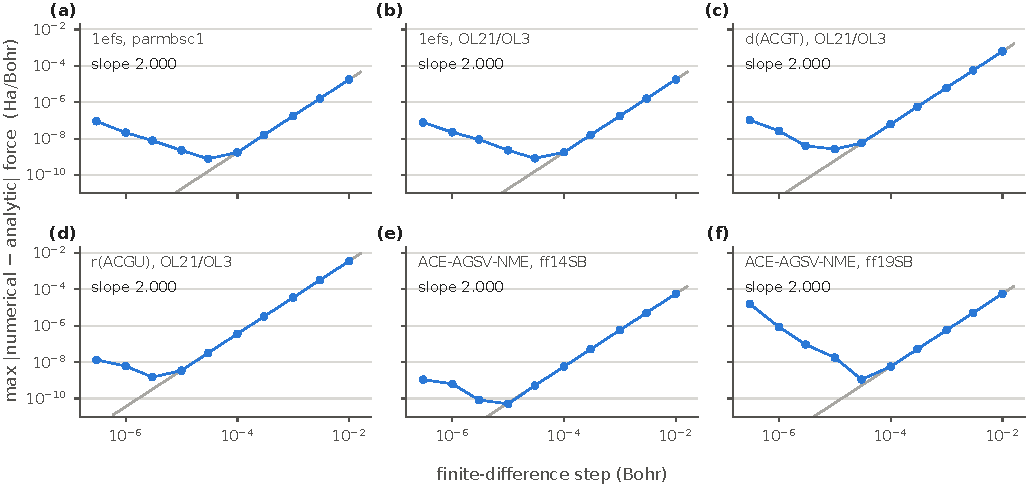
\includegraphics[width=\linewidth]{force-convergence.pdf}
\caption{Convergence of the central-difference check on the total-energy
gradient for six of the 61 sweeps, one per Cartesian system and force field.
Each point is the largest $|$numerical $-$ analytic$|$ force component over all
atoms at that step. The grey line has slope exactly 2 through the coarsest
point; the printed exponent is the least-squares fit over the fixed window
$10^{-2}$ to $3\times10^{-4}$~Bohr. Below the window each sweep leaves the
falling branch where round-off in the energy overtakes the discretisation
error, which is a floor and not a disagreement. Source:
\texttt{evidence/forces/*.all.tsv}.}
\label{fig:force-convergence}
\end{figure}

A residual at a given step is not an error in the force. It is dominated by the
discretisation error of the difference at coarse steps and by round-off in the
energy evaluation at fine ones, and it is smallest where the two cross. At the
coarsest step, $10^{-2}$~Bohr, residuals across the set run up to
$3.6\times10^{-3}$~Ha/Bohr, which is what a central difference of that width
is expected to give. The number worth quoting is the minimum over each sweep.
The largest of the 61 minima is $3.8\times10^{-9}$~Ha/Bohr, on the non-bonded
staging gradient of the RNA 4-mer; the smallest is $4.5\times10^{-13}$, on the
peptide torsion under ff19SB. For scale, 0.002~\kcal{} per Bohr is
$3.2\times10^{-6}$~Ha/Bohr, and every one of the 61 minima is smaller than that
by a factor of at least 800.

The exponent is the measurement, and it was fitted over a step window fixed in
advance instead of chosen per sweep: $10^{-2}$ to $3\times10^{-4}$~Bohr, the
four coarsest steps, which every one of the 61 sweeps spans. Over that window
the fitted exponents run from 1.994 to 2.009, with a mean of 2.000 and a
standard deviation of 0.002. The fits are tight: the largest root-mean-square
residual of any of the 61 is 0.003 in $\log_{10}$ of the force residual, and no
single point departs from its own fit by more than 0.005. That is the
second-order convergence a central difference gives when the analytic force
really is the derivative of the energy. Below the window every sweep leaves the
falling branch at its own step and flattens, which is round-off and not
disagreement; the correction map leaves it earliest and climbs again, reaching
$1.6\times10^{-5}$~Ha/Bohr at $3\times10^{-7}$~Bohr, because the map is
interpolated on a grid and is not smooth to machine precision.

The sweep found one defect that no energy comparison in this paper could have
found. The correction-map analytic force was identically zero at a dihedral of
exactly $\pi$, which is where a peptide built extended sits; it is fixed and
pinned by a test (F-21). The energy was never affected, and every sweep
reported here is post-repair.

\subsection{What one Monte Carlo step costs}
\label{sec:cost}

One Monte Carlo step on the 818-atom heteroduplex under OL21/OL3 costs
3.46~ms on one core of an Apple M5 laptop, with 449~ms of setup that happens
once per run; the linear fit over $N = 0$ to $100$ steps has $R^2 = 0.99968$
(Figure~\ref{fig:cost-fit}). A step is one torsional proposal plus one full
energy evaluation over every non-excluded pair, so the figure is an upper bound
on the energy evaluation alone; the proposal is inside it and is not separated
here. It is a cost, not a benchmark: nothing here compares MOSAICS with another
program on the same hardware, the engine has never been tuned for the speed of
a single evaluation, and the number says nothing about scaling or about other
sizes. What it settles is the question a reader of the 26-cell matrix is
entitled to ask next, which is what one of those evaluations costs when the
engine is actually sampling. The strength the method claims lies elsewhere, in
the number of evaluations a guided proposal needs to cross a barrier that
molecular dynamics must climb in femtosecond steps, and that ratio is not
measured in this paper.

\begin{figure}[tbp]
\centering
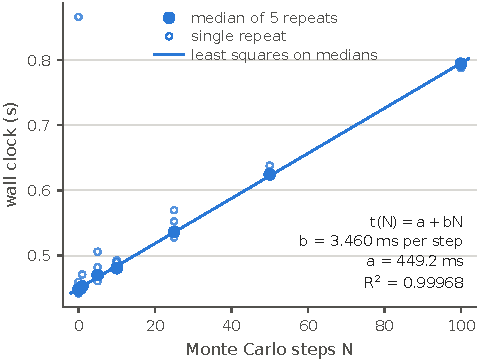
\includegraphics[width=0.5\linewidth]{cost-fit.pdf}
\caption{Wall clock against number of Monte Carlo steps for the committed
1efs OL21/OL3 input, 818 atoms, serial, one core of an Apple M5. Small hollow
markers are the five repeats at each $N$, filled markers their medians, the
line the least-squares fit to the medians. The one 866~ms outlier at $N=0$ is
why medians are used. Source:
\texttt{work/preprint-I/runs/2026-08-31-cost-818/result.json}, re-fitted by
\texttt{figures/cost-fit.py}, which exits if its fit disagrees with the
committed one.}
\label{fig:cost-fit}
\end{figure}

\subsection{\studio{}: the same engine, verified in the browser}
\label{sec:studio-results}

The Studio is only as good as the engine it carries, so its verification is of
the same kind as the rest of this paper: the same input, run under the native
engine and under the WebAssembly one, compared number by number.
Figure~\ref{fig:studio} shows the page at two of its four steps on the run used
for that check.

\begin{figure}[p]
\centering
\begin{subfigure}[t]{0.84\linewidth}
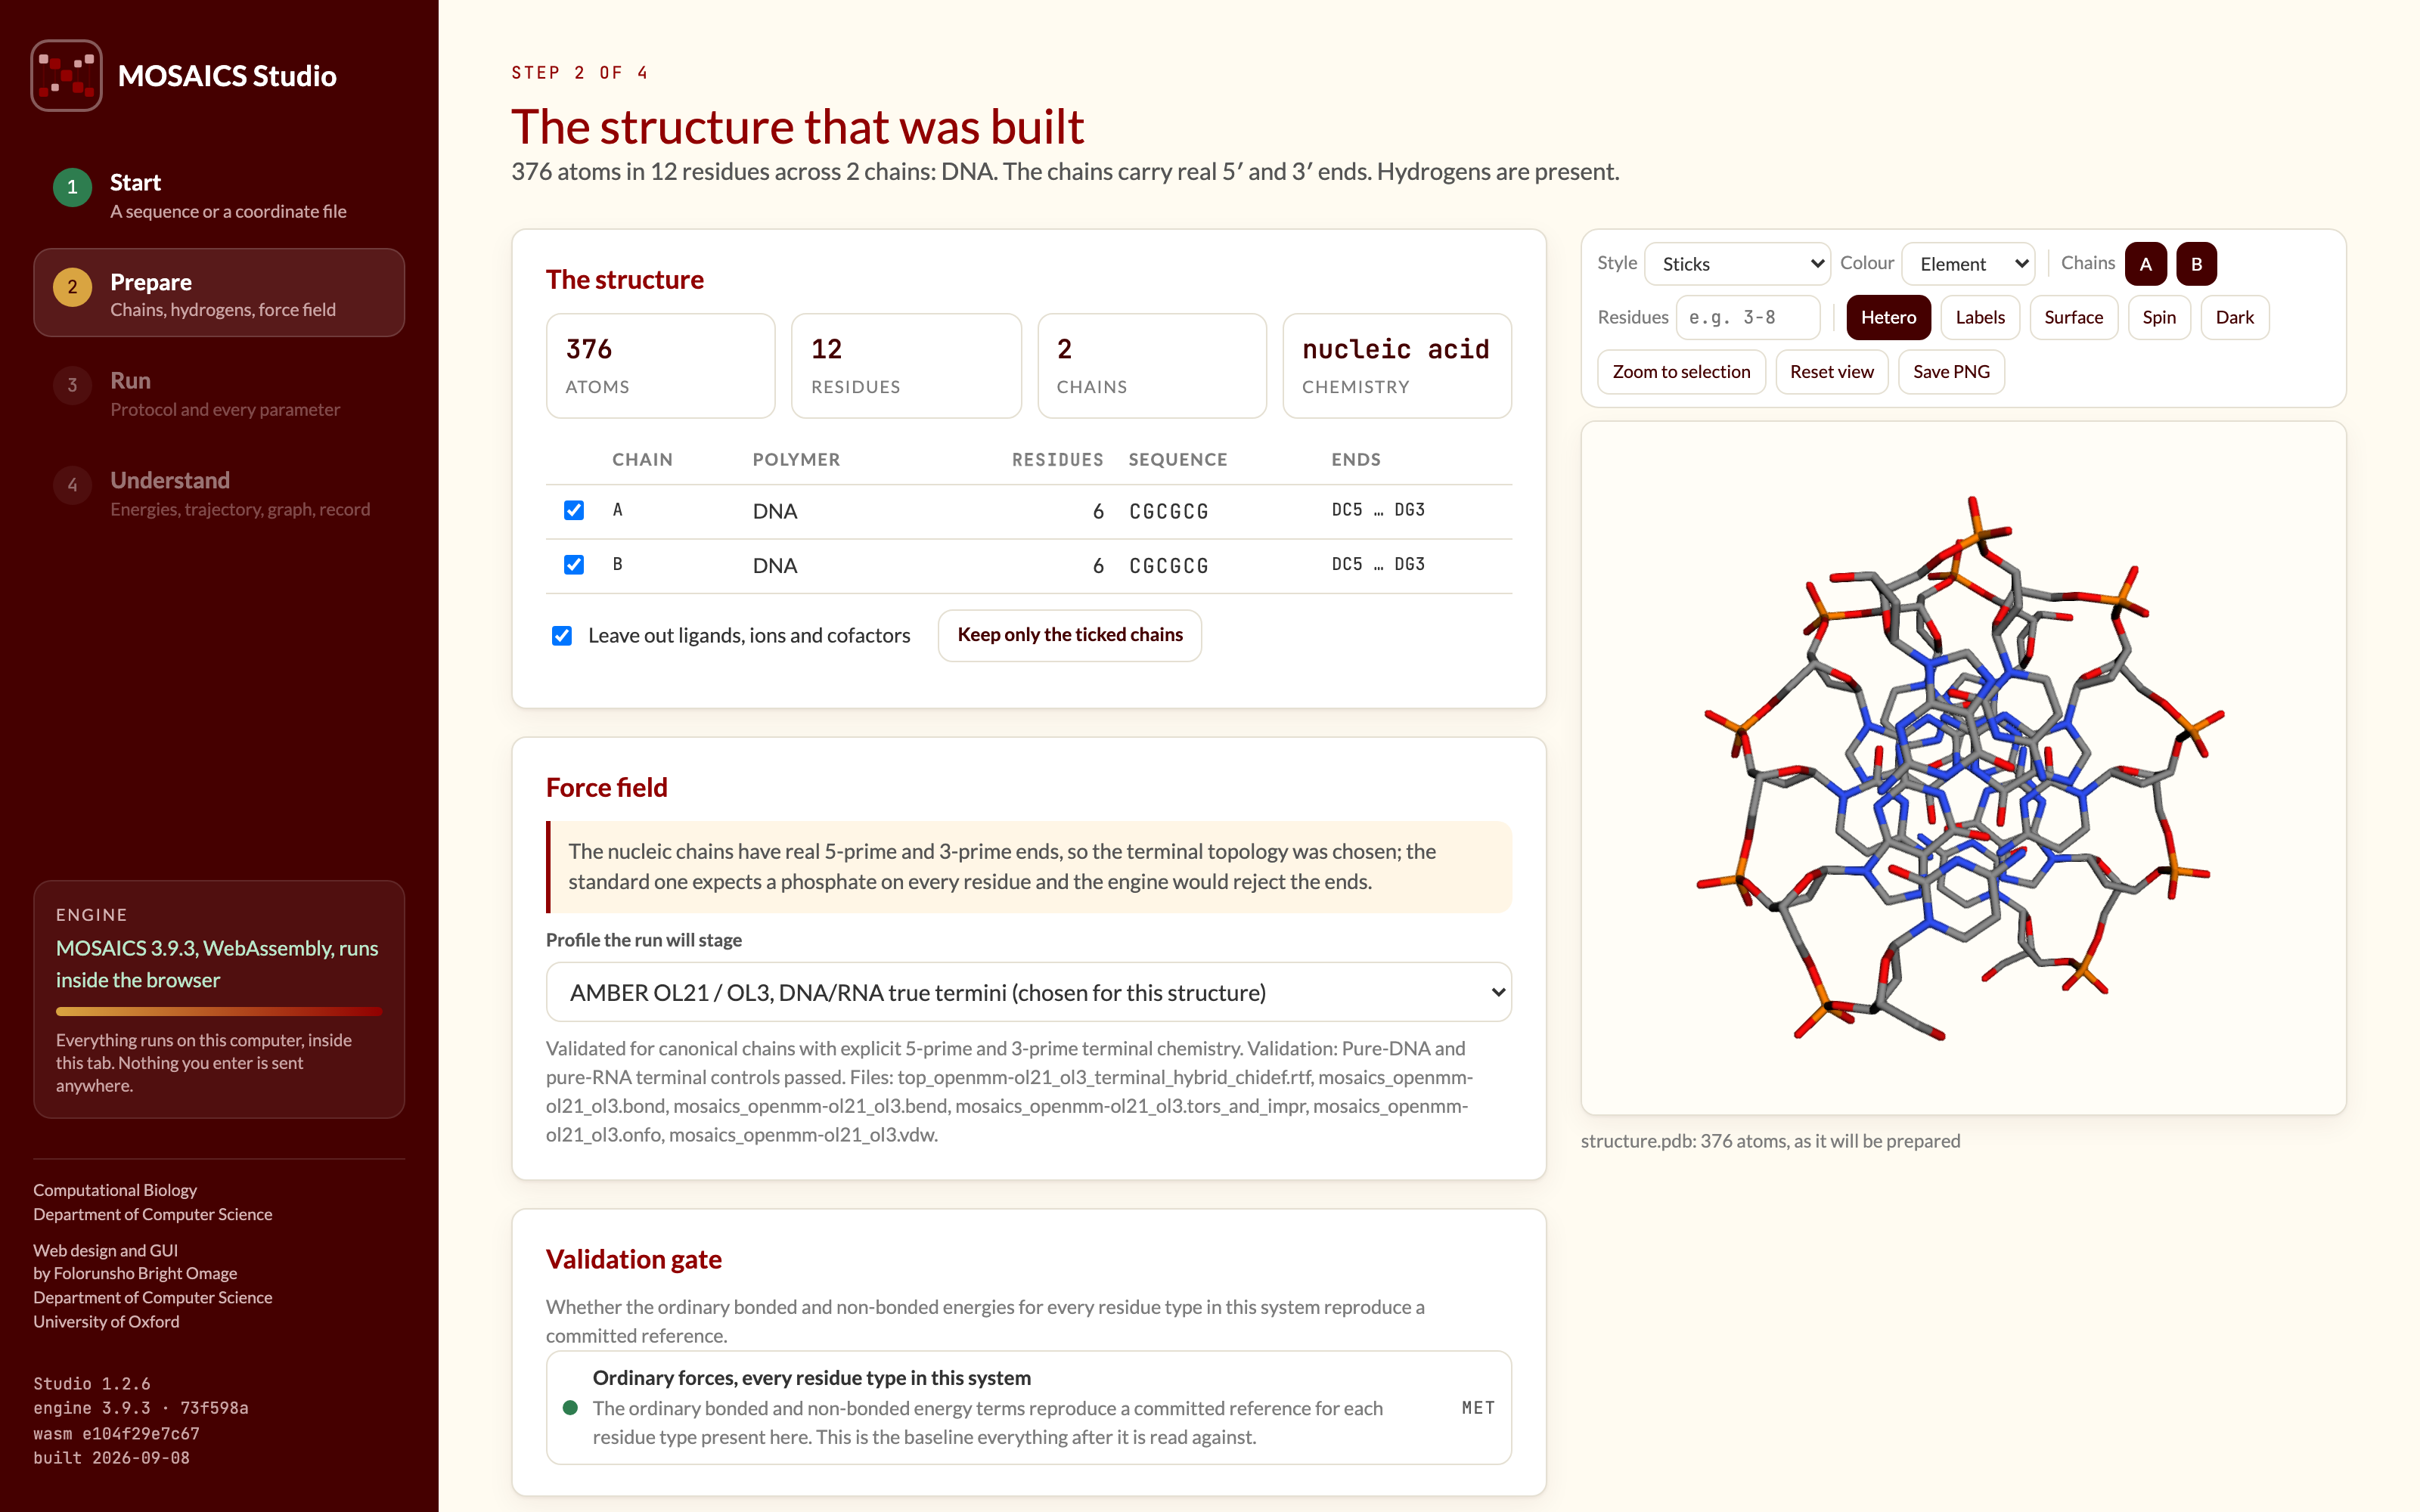
\includegraphics[width=\linewidth]{studio-prepare.png}
\caption{}
\label{fig:studio-prepare}
\end{subfigure}
\par\smallskip
\begin{subfigure}[t]{0.84\linewidth}
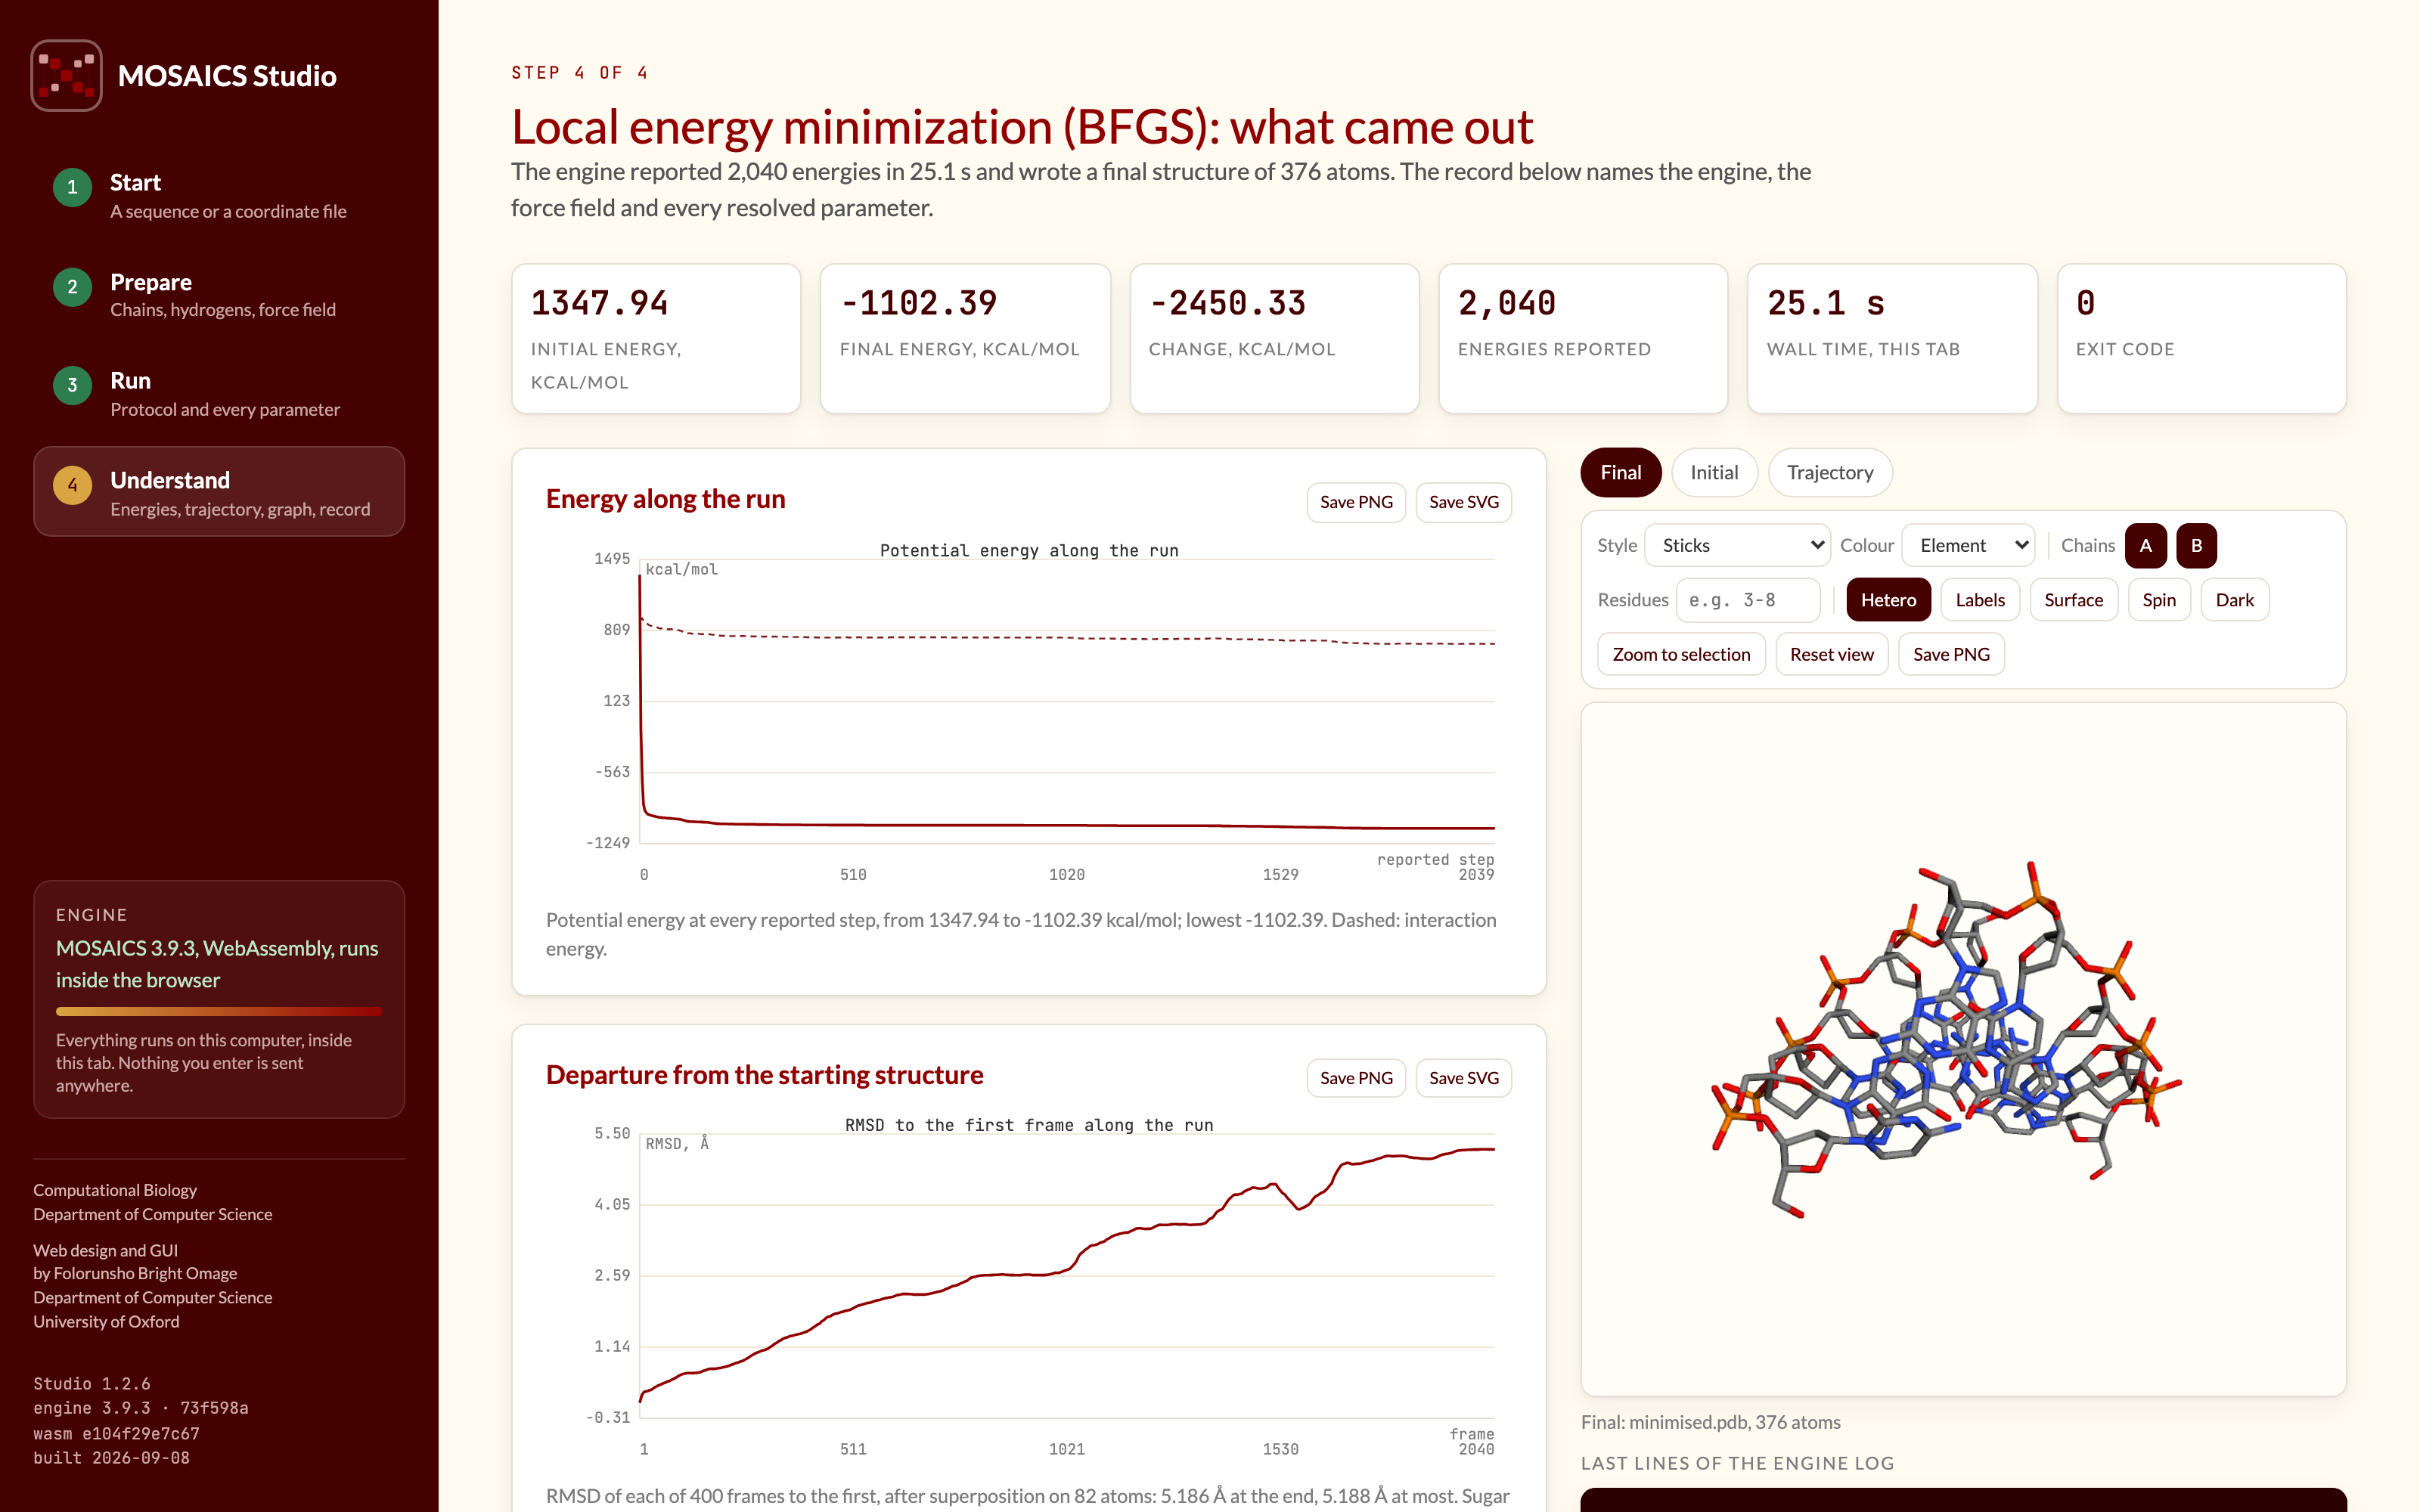
\includegraphics[width=\linewidth]{studio-understand.png}
\caption{}
\label{fig:studio-understand}
\end{subfigure}
\caption{\studio{} in the browser, version 1.2.6, on the CGCGCG duplex used
for the cross-check of Table~\ref{tab:studio}. (a) The Prepare step: the built
structure, 376 atoms in 12 residues across two chains with real $5'$ and $3'$
ends; the force field chosen with its reason, here the OL21/OL3 terminal deck
because the chains carry real ends; the validation gate reporting that the
ordinary bonded and non-bonded energies for every residue type present
reproduce a committed reference; and the 3Dmol.js viewer. The left rail names
the engine as WebAssembly running inside the tab, with the Studio version,
engine commit, engine digest and build date. (b) The Understand step after the
BFGS minimisation: initial and final energies, the number of energies
reported, the wall time in this tab and the exit code; energy along the run;
RMSD to the first frame along the trajectory; and the final structure. The
energy-against-RMSD plot, the residue-by-residue comparison, the graph export
and the record follow further down the page. The Start and Run steps are in
Supporting Information Figure~S1.}
\label{fig:studio}
\end{figure}

\paragraph{Native against WebAssembly}
The Studio's documented case study builds CGCGCG as a B-DNA duplex, minimises
it with the \texttt{local-minimum} preset (BFGS to a gradient tolerance of
$10^{-7}$) on the OL21/OL3 terminal deck, exports a residue graph and writes
the report. Replaying the deck the Studio writes under the native Apple-silicon
engine and under the WebAssembly engine gives Table~\ref{tab:studio}: the same
exit code, the same 2,040 BFGS iterations, the same first and last energies to
the two decimals the engine's energy file carries, a largest difference along
the series of 0.25~\kcal{}, and a final-structure RMSD of 0.0045~\AA{} between
the two. A headless test drives the whole pipeline, the same Python archive and
the same bridge the page uses, and fails unless those numbers reproduce. The
run in Figure~\ref{fig:studio} is that case study executed on the live page in
a headless Chromium session on 8 September 2026: 2,040 energies reported,
1347.94 to $-1102.39$~\kcal{}, 25.1~s of wall time in the tab against 20.8~s
under Node and 11.5~s for the native engine.

\begin{table}[t]
\centering
\small
\caption{The CGCGCG case study replayed under the native engine and under the
WebAssembly engine, from the Studio's build record. The native binary is the
Apple-silicon 3.9.1 build at engine commit \texttt{ea00b02}; the WebAssembly
build is from commit \texttt{73f598a} (7 September 2026). Source:
\texttt{web/engine/BUILD.md} in the Studio repository.}
\label{tab:studio}
\begin{tabular}{@{}lrr@{}}
\toprule
 & native, arm64 & WebAssembly \\
\midrule
exit code & 0 & 0 \\
BFGS iterations reported & 2040 & 2040 \\
first energy (\kcal{}) & 1347.94 & 1347.94 \\
last energy (\kcal{}) & $-$1102.39 & $-$1102.39 \\
largest difference along the series (\kcal{}) & \multicolumn{2}{c}{0.25} \\
final-structure RMSD (\AA{}) & \multicolumn{2}{c}{0.0045} \\
wall time, Node 26 (s) & 11.5 & 20.8 \\
\bottomrule
\end{tabular}
\end{table}

\paragraph{The record}
The run in Figure~\ref{fig:studio}(b) wrote a record naming Studio 1.2.6, the
engine commit \texttt{73f598a} and the SHA-256 of the WebAssembly build, the
six staged files of the OL21/OL3 terminal deck by digest, the preset and every
parameter it resolved, and the start and end times, with the final structure,
the engine deck, the engine log, the energy series and the trajectory beside
it, each one click away. That record is what a reader who repeats the run
compares against, and it is the same document on every machine that loads the
page, because no part of the computation happens anywhere else.

\section{Discussion}
\label{sec:discussion}

\subsection{What an additive all-atom energy makes available}
\label{sec:whatchanges}

The sampling half of natural-move Monte Carlo is unchanged by any of this. What
changes is what an accepted structure is worth. A knowledge-based potential
returns a ranking: it says which of two models is preferred, on a scale fitted
to that comparison and to the representation it was fitted on
\cite{minary2008foldspace,leaverfay2011rosetta}. For structure prediction, and
for refinement where an experimental restraint carries most of the signal
\cite{zhang2012multiscale,chang2020rnacryoem}, that is sufficient. It is not
sufficient for anything that needs the energy itself. Two such numbers computed
for two different molecules do not lie on the same axis, nothing computed from
the energy on an absolute scale is available, and a structure cannot pass
between the Monte Carlo engine and a molecular dynamics run without the sampled
quantity changing definition on the way.

With eight parameter families evaluated to the tolerances of
Sections~\ref{sec:matrix} and~\ref{sec:energies}, those obstructions are lifted
for the chemistry and the geometries tested, and for nothing beyond them. The
claim the data supports is narrow and should be stated narrowly: handed a
published deck, the engine reproduces that deck's energy and its gradient to
the tolerance reported, whichever deck it is. The four AMBER nucleic decks are
substantially different parameter sets, and the engine follows each of them
without being retuned for any. What that does not license is a statement about
how far apart the decks put a molecule. A Fourier torsion sum, $\sum
(V_n/2)[1+\cos(n\phi-\gamma)]$, does not vanish at any reference state, and a
refit moves its additive constant as freely as it moves its shape; the
quantity that would carry that argument is $\Delta\Delta E$ between at least
two conformations of the same molecule under two decks, and it is not computed
here.

What the engine can now be asked, for the systems tested, is a different class
of question. It can be run at a stated temperature against a named force field,
so that an ensemble it produces and an ensemble a molecular dynamics code
produces under the same parameters are ensembles of the same function; and a
configuration produced by a collective move can be continued under molecular
dynamics, or taken from one, without the energy being redefined in between.
Neither is demonstrated in this paper. What is demonstrated is the
precondition: the energy and its gradient are the published ones, at the
geometries and on the chemistry tested.

\subsection{What the extension to eleven systems adds, and what it does not}
\label{sec:elevenadds}

The two reference systems of Section~\ref{sec:energies} settle whether the
engine evaluates a deck correctly, term by term, against three programs. The
other nine settle a different question: whether it does so on the chemistry a
user will actually bring. A deck is a few hundred to a few thousand parameter
rows and a 56-atom peptide reaches a fraction of them. Ubiquitin, BPTI and the
MHC heavy chain between them select every amino-acid type ff14SB and ff19SB
carry, with charged, aromatic, histidine and proline residues, disulfides and
charged termini; the dodecamer and the tetraloop select all eight bases and both
$5'$-OH and $3'$-OH ends; the two complexes select a bound peptide in a groove
and a protein--RNA interface. That every one of those cells lands within a few
thousandths of a \kcal{} of the references, and that the two that land further
away resolve to the atom order of a single improper, is what the extension
adds.

It also sharpens what the residuals mean. On the two reference systems the
angle term carried the largest residual and it was attributed to the reference
topology (F-12). Seven further systems now carry the same residual with the
same sign, growing with the number of angles, which is what a rounding of
$\pi/180$ in the topology builder predicts and what a defect in the engine's
bend routine would not. The improper cells make the complementary point: the
one large disagreement in the matrix is not a parameter or an expression but a
convention, the order in which four atoms are listed, and it appears where the
geometry departs from planarity and nowhere else. Cross-engine agreement
certifies the evaluation path. It does not certify the path that produced the
parameters, and both of the residuals that survive at the top of the matrix
live there.

What the extension does not add is a per-term comparison against all three
references for every cell. The totals are against two or three programs on 20
of the 26 cells and against OpenMM alone on the other six; the per-term
resolution in Figure~\ref{fig:energy-agreement}(b) exists only where the output
files carry it, and eleven OpenMM comparisons print a single non-bonded sum.
Nor does it add a second conformation per system. The extension widens the
chemistry and holds the geometry fixed, and the failure mode F-21 demonstrates
remains open on every cell.

\subsection{What changed in the engine, and what did not}
\label{sec:baseline}

A reader is entitled to know how much of this is new code, because that is
where the risk of a new defect lives. The honest answer is that most of it is
not. Both CHARMM-specific terms were carried on machinery the engine already
had. The 1497 Urey--Bradley entries in CHARMM36 reduce to 810 unordered
triples, of which 807 are written into the bond slot of the existing bend
record, which \texttt{bend.cpp} already evaluates as
$\tfrac{1}{2}k(r_{13}-r_0)^2$, the functional form CHARMM asks for; three
triples are dropped and counted, because four P--ON2--P variants carry negative
force constants that CHARMM permits and the deck reader rejects, and they are
pyrophosphate linkages that do not occur in a phosphodiester backbone (F-16).
The 188 harmonic impropers are carried on the existing torsion record with
\verb|\pot_type{harm}|, which the deck reader expands onto the same power series
it uses for the cosine form. That expansion is a genuine approximation, exact
to four figures at $10^{\circ}$ from equilibrium and $-7.7$\,\% at
$60^{\circ}$, and the ten-digit agreement reported for the improper term is at
a total of $1.0\times10^{-3}$~\kcal{}, where the series and the quadratic
coincide by construction.

Where the defects were was the converter and, in a few places, the engine. The
CHARMM XML splits the non-bonded term between two elements, charge in
\texttt{NonbondedForce} and $\sigma$, $\epsilon$ in
\texttt{LennardJonesForce}; the converter read only the first, so an entire
CHARMM deck carried $\epsilon = 0$ on all 85\,078 pair entries. The
correction-map analytic force was identically zero at $\phi = \pi$, because a
$\sin\phi$ clamp replaced a vanishing denominator and left a vanishing
numerator (F-21); it is now written in the form with no $\sin\phi$ in it. Forty
arrays allocated with \verb|new[]| were grown with \verb|realloc| (F-19), which
ran on every committed job and was invisible because the relevant sanitizer
check is off by default on macOS. And the deck reader now carries the
per-molecule torsion label and chains the residues it builds; the released
3.9.1 refuses the decks that need the first and returns energies tens of
thousands of \kcal{} from the references without the second.

The novelty is not all-atom Monte Carlo on an additive force field. That
exists: CAMPARI with ABSINTH, MCPRO and BOSS, ProtoMS and Cassandra all evaluate
all-atom additive potentials under Metropolis Monte Carlo, and concerted-rotation
move sets have been run in OPLS for both protein and nucleic acid backbones
\cite{ulmschneider2003concerted,ulmschneider2004concertedna,vitalis2009mcmethods}.
What is new here is the pairing of that energy with the nested natural-move
hierarchy and its stochastic chain closure
\cite{minary2010chainclosure,sim2012naturalmoves}, so that one proposal can act
at the scale of a domain and the next at the scale of a sugar pucker while the
accepted energy stays a published one, and the delivery of that pairing to a
user who has never seen the engine's input syntax. The claim is the combination,
and it should be read that way.

\subsection{Three references, and what the third one pays for}
\label{sec:threerefs}

Agreement with a single reference program is a weaker claim than it looks. It
establishes that two codes treat a parameter file the same way, which confounds
correct evaluation with shared convention: the same choice of 1--4 scaling, the
same grouping of impropers, the same charge-to-energy constant. Three
independently written programs break that confound in both directions. Where
they agree with one another, the target is not in dispute and a residual
against any of them is a measurement of the implementation. Where they
disagree, the disagreement is itself a number, and it bounds what any
cross-engine claim can resolve. On 1efs the bound is $2.6\times10^{-5}$~\kcal{}
on Lennard-Jones and $3.4\times10^{-5}$ on electrostatics, which is what OpenMM
and GROMACS return against each other when handed the same parameters and the
same coordinates through the ordinary conversion route.

Each of the two convention differences reported here was invisible to some
subset of the three. The GROMACS route is the only one that could not carry
ff19SB's per-residue correction maps, and running it put a number on what that
costs: 0.30~\kcal{} on a four-residue peptide and 8.4~\kcal{} on ubiquitin, from
applying one residue's map to every residue. sander, separately, is the only one
of the three that does not share the modern charge-to-energy constant, and a
comparison against OpenMM and GROMACS alone would have shown MOSAICS's own
$8.2\times10^{-7}$ offset while leaving the $3.5\times10^{-5}$ carried by a
widely used engine undetected. Neither is a defect in the engine that exposed
it, and neither would have been found by adding a fourth code from the same
family. The independence is in the code and not in the input, and that limit is
worth stating because it is where the argument is weakest: all three references
read a topology written by one builder, so an error in the builder appears
identically in all three, and F-12 is exactly that case. The three references
are also not of equal weight: six combinations against three engines, fourteen
more against two, and six against OpenMM alone are not the same strength of
claim, and Table~\ref{tab:matrix} keeps them apart.

\subsection{The charge-to-energy constant is a general hazard}
\label{sec:constantgeneral}

The constant that converts $q_iq_j/r$ into \kcal{} is not the same number in
every program, and any group differencing energies across programs is exposed
to that. sander uses $18.2223^2 = 332.052217$, an older value carried in the
way it stores topology charges; OpenMM and GROMACS both return $332.063713$
from the same two-charge measurement. The relative gap is $3.5\times10^{-5}$,
which on the 1efs electrostatic term of 1857.7~\kcal{} is 0.064~\kcal{}, roughly
360 times the largest residual this work is trying to resolve and about a tenth
of $kT$ at 300~K. The constant enters multiplicatively, so it does not cancel
when two conformations of the same molecule are compared: it biases the
electrostatic part of that difference by the same $3.5\times10^{-5}$, and its
absolute size grows with the electrostatic energy, which is to say with system
size and with net charge. It also has nothing to do with the AMBER family: the
same offset accounts for the CHARMM36 residuals on every one of the five
CHARMM36 cells, and once it is removed those cells are the closest agreement in
this work, at a few parts in $10^{12}$ of the term. The practical
recommendation is to measure the constant instead of taking it from
documentation, which is a few minutes of work in any engine that will read a
topology, and to state which constant a comparison was corrected to, because
the choice is worth $1.7\times10^{-6}$~\kcal{} on this system.

\subsection{What these numbers do not establish}
\label{sec:limits}

The first limit is the one conformation. Every run sets all proposal widths to
zero, so a term that happens to vanish at that geometry is untested. The capped
peptide sits at the minimum of its out-of-plane terms and both MOSAICS and
GROMACS return zero for them (F-11). More seriously, the correction-map
analytic force was identically zero, 0 of 168 components, because a peptide
built extended sits at $\phi = \psi = \pi$, the singular point of the
implemented expression, and \emph{every energy comparison on that system passed
while that was true} (F-21). It took a gradient sweep to find it. The same
failure mode is available to any term whose parameter is wrong but inactive, or
whose phase is wrong but degenerate, at the one geometry tested, on any of the
26 cells. Repeating these single points over 50 to 100 decorrelated snapshots
per system, as Shirts \emph{et al.}\cite{shirts2017engines} do, would close it,
and it is cheap on vacuum systems of this size. It has not been done here.

The second is that the force sweeps cover four systems and the term-by-term
comparison two. The nine added systems carry totals, and per-term differences
where the output files resolve them, but no force sweep and no staged sweep.
The correction map is exercised at the force level on one system, because the
ff19SB peptide is the only committed force input that loads a map database and
no nucleic parameter set here carries one (F-22).

One committed structure is geometrically defective and the defect is not
repaired. In \path{examples/pure_terminal_controls/dna_acgt.pdb}, residue DG~3,
H5$'$ and H5$''$ each sit 1.089 and 1.090~\AA{} from C5$'$, which is right, and
0.060~\AA{} from each other, which makes the H--C--H angle $3.15^{\circ}$
instead of $109.5^{\circ}$ (F-17). The offending pair is 1--3, which the
non-bonded sum excludes, so no energy check sees it as an error; the symptom is
that this 126-atom 4-mer returns a bend energy of 508.62~\kcal{} under the AMBER
decks against 220.56 for the 818-atom heteroduplex, and 412.79 under CHARMM36
against 166.36 for the RNA 4-mer of the same size. The cross-engine comparison
is unaffected, because every program reads the same coordinates and they
reproduce each other on them. The file was pinned in a test and left alone
because committed reference tables were computed from it; repairing it and
regenerating those tables is the right fix and has not been done.

Three scope limits belong with these. CHARMM36 for protein is not available in
MOSAICS, and the obstruction is a file format and not a physical one: its
correction maps are selected partly by the residue that follows the one being
corrected, while the engine's map-selection record keys on the residue itself
(F-09), and no claim about the CHARMM36 protein parameters
\cite{best2012charmm36,huang2017charmm36m} appears anywhere in this work. Two
decks cannot be regenerated from their sources (F-20), so the seventh decimal
of the OL15/OL3 and OL21/OL3 bonded terms is reporting transcription; and the
OL24 parameter files come from a package whose redistribution terms are its
authors', so a reader who does not hold that package cannot rebuild those three
cells from a clone. And parmbsc1 has no terminal deck and parmbsc0 does not run
on a free-ended duplex, which is why the dodecamer has no cell under either.

There is a gap between the code path validated here and the code path a
production run executes, and it is narrower than that sentence usually implies.
MOSAICS scores a proposal by recomputing the whole potential, so the term
routines checked here are the term routines a proposal is judged by. What no
single point exercises is a choice of pair set: \texttt{inter\_list} is
\texttt{none} in every committed input, so the link-list and neighbour-list
branches never ran. Closing that costs one single point per branch with a list
cutoff longer than the molecule, differenced against the numbers reported here
to the summation-order tolerance of $5.5\times10^{-11}$~\kcal{}. Neither run is
in this paper.

Single-point energies and finite-difference force checks fix the value of the
energy function at a geometry and its gradient there. They say nothing about
whether the move set, the stochastic chain closure and the acceptance rule
together generate the Boltzmann distribution of that energy
\cite{minary2010chainclosure,hatch2025mcbestpractices}; that is a separate
validation with separate diagnostics, and it is not attempted here. The cost
figure of Section~\ref{sec:cost} is likewise not an efficiency result: a
per-step time on one machine compares nothing with anything, and the quantity
that would, sampling per unit cost against a molecular dynamics baseline on the
same system and the same force field, is the next measurement and not this
one. Nor do these numbers speak to whether ff19SB or OL21/OL3 is right about a
molecule, which is measured against experiment and not against another program
\cite{lindorfflarsen2012validation,beauchamp2012benchmark,love2023amberdna}.
And everything was run in vacuum at dielectric~1 with no cutoff, so no cutoff
scheme, switching function or implicit-solvent term is covered by any number in
this paper.

\subsection{What the Studio does and does not establish}
\label{sec:studio-limits}

The Studio's verification is of the engine it carries, on one documented run.
The cross-check shows that the WebAssembly build follows the native one through
2,040 minimisation steps to the same energies at the precision the energy file
carries and to 0.0045~\AA{} in the final structure; it does not show that every
protocol behaves identically in the browser, and two protocols are known to
differ by construction, because the browser engine is single-threaded and
parallel-tempering replicas take turns. The record binds what ran to what was
produced; it does not make the run correct, and the validation gate on the
Prepare step checks the ordinary energy terms of the residue types present
against a committed reference, which is the baseline of this paper and not
more. No external user has run the software at the time of writing, and
proteins are prepared from coordinates rather than built.

\subsection{Next}
\label{sec:next}

The intended application is conformational sampling of peptide--MHC complexes,
and it is the next piece of work rather than a result reported here. The system
suits the move set: a bound peptide with a small number of internal degrees of
freedom in a groove, flanked by domains that move as units, which is the
granularity natural moves were built for \cite{sim2012naturalmoves}, and
hierarchical natural-move Monte Carlo has already been applied to peptide
dissociation from MHC class~I \cite{knapp2016pmhc}. What exists in this work is
the implementation side of that study: the complex evaluates under both
protein force fields to within 0.005~\kcal{} of two references at 6,139 atoms,
the staging transform was checked on a peptide--MHC fixture at the gradient
level, and the Studio will prepare and run it. No sampling run of any kind on
that system appears in the evidence.

Several things should be settled before such a study is worth reporting, and
each is small and named. The single points should be repeated over an ensemble
of decorrelated configurations per system, the only cheap defence against the
failure mode F-21 demonstrates. The force sweeps should be extended to the nine
added systems. The two large cells that are not resolved into terms should be.
The link-list and neighbour-list branches of the non-bonded sum need the two
single points described above. The defective control structure should be
repaired and its reference tables regenerated (F-17); the two decks that cannot
be regenerated should be rebuilt (F-20); the peptide needs a deliberately
distorted copy so that the out-of-plane terms and the CHARMM improper series
are exercised away from their minima (F-11). Beyond the fixtures, the certified
regime has to be widened from vacuum with no cutoff to whatever solvent
treatment a production run will use, which is a further round of the same
term-by-term comparison and not an extrapolation from these numbers. The
criterion for judging the study that follows should not be whether the Monte
Carlo engine reproduces a molecular dynamics trajectory. It should be whether
the engine reaches configurations that molecular dynamics does not reach in
comparable time, at energies that mean the same thing in both. The present
paper speaks only to the second half of that sentence, and only on the
chemistry and the geometries it tested.

\section{Availability}
\label{sec:availability}

\paragraph{\studio{}}
The page is served as static files at
\url{https://users.ox.ac.uk/~coml1155/mosaics-studio/} and needs a current
Chrome, Edge, Firefox or Safari with WebAssembly and Web Workers, about 25~MB on
first visit and a few hundred megabytes of memory during a run; the version
described here is 1.2.6. The source is at
\url{https://github.com/omagebright/mosaics-studio} under the MIT licence. The
page carries the MOSAICS engine compiled to WebAssembly, redistributed with the
permission of the engine's author; the force-field data are distributed as
separate works and the underlying parameter sets should be cited to their
original publications, which Section~\ref{sec:methods-parameters} names.

\paragraph{The engine}
MOSAICS \cite{mosaics-software} is developed at
\url{https://www.cs.ox.ac.uk/mosaics/}. The evaluation code, the deck reader,
the converters that write the decks, the reference builders and every
single-point input used here live in the engine's source distribution, with
the decks under \texttt{params/} and the structures under \texttt{examples/},
and the inputs and outputs behind every number in this paper are kept in the
evidence tree that accompanies the manuscript sources, one directory per force
field and system. That distribution is at present cited by name and project
page: it carries no DOI and no public release tag, so a reader cannot yet fetch
the exact tree these numbers came from. An archived, versioned deposit with a
licence statement is needed and does not yet exist; it is the largest single
obstacle to reproducing this paper, and closing it means publishing an
artefact, not running anything again.

\paragraph{Manuscript, evidence and data}
The manuscript sources, the scripts that draw every figure and table, the two
data files behind the tables and both evidence trees are deposited at Zenodo
under DOI 10.5281/zenodo.22661461 and developed at
\url{https://github.com/omagebright/mosaics-studio-preprint}, under the
CC~BY~4.0 licence.

\paragraph{Supporting Information}
The MOSAICS single-point settings, the deck sizes, the reference-engine control
files, the four 1efs \texttt{tleap} presets, the commands that read each
engine's output, the CHARMM36 conversion route, the 1efs coordinate edits, and
the Start and Run steps of the page.

\section*{Acknowledgements}
The force-field parameter sets are the published work of their authors, cited
in Section~\ref{sec:methods-parameters}; the reference calculations were made
with AmberTools, OpenMM and GROMACS as distributed. F.B.O. thanks the
Department of Computer Science, University of Oxford, for hosting the visit
during which this work was done.

\section*{Author contributions}
F.B.O. converted the parameter sets, built the reference calculations and the
evidence tree, wrote \studio{} and its browser build, and drafted the
manuscript. P.M. wrote the
MOSAICS engine and the natural-move method, directed the scope and the
verification strategy, and revised the manuscript.


% Hand-written bibliography, so that no BibTeX run is needed. Every journal
% entry was checked against the publisher-deposited Crossref record at the DOI
% given; the six Protein Data Bank primary citations were read from the RCSB
% entry records and then checked at Crossref. Software without a paper is
% cited as software with a URL and an access date. Order follows first
% appearance in the text.
\begin{thebibliography}{99}
\small
\setlength{\itemsep}{1pt}

\bibitem{dror2012microscope}
R.~O. Dror, R.~M. Dirks, J.~P. Grossman, H.~Xu, and D.~E. Shaw,
``Biomolecular simulation: a computational microscope for molecular biology,''
\emph{Annu. Rev. Biophys.} \textbf{41}(1), 429--452 (2012).
DOI: 10.1146/annurev-biophys-042910-155245.

\bibitem{shaw2010anton}
D.~E. Shaw, P.~Maragakis, K.~Lindorff-Larsen, S.~Piana, R.~O. Dror,
M.~P. Eastwood, J.~A. Bank, J.~M. Jumper, J.~K. Salmon, Y.~Shan, and
W.~Wriggers,
``Atomic-level characterization of the structural dynamics of proteins,''
\emph{Science} \textbf{330}(6002), 341--346 (2010).
DOI: 10.1126/science.1187409.

\bibitem{lindorfflarsen2011folding}
K.~Lindorff-Larsen, S.~Piana, R.~O. Dror, and D.~E. Shaw,
``How fast-folding proteins fold,''
\emph{Science} \textbf{334}(6055), 517--520 (2011).
DOI: 10.1126/science.1208351.

\bibitem{torrie1977umbrella}
G.~M. Torrie and J.~P. Valleau,
``Nonphysical sampling distributions in Monte Carlo free-energy estimation:
umbrella sampling,''
\emph{J. Comput. Phys.} \textbf{23}(2), 187--199 (1977).
DOI: 10.1016/0021-9991(77)90121-8.

\bibitem{sugita1999remd}
Y.~Sugita and Y.~Okamoto,
``Replica-exchange molecular dynamics method for protein folding,''
\emph{Chem. Phys. Lett.} \textbf{314}(1--2), 141--151 (1999).
DOI: 10.1016/S0009-2614(99)01123-9.

\bibitem{laio2002metadynamics}
A.~Laio and M.~Parrinello,
``Escaping free-energy minima,''
\emph{Proc. Natl. Acad. Sci. U.S.A.} \textbf{99}(20), 12562--12566 (2002).
DOI: 10.1073/pnas.202427399.

\bibitem{bernardi2015enhanced}
R.~C. Bernardi, M.~C.~R. Melo, and K.~Schulten,
``Enhanced sampling techniques in molecular dynamics simulations of biological
systems,''
\emph{Biochim. Biophys. Acta Gen. Subj.} \textbf{1850}(5), 872--877 (2015).
DOI: 10.1016/j.bbagen.2014.10.019.

\bibitem{minary2010chainclosure}
P.~Minary and M.~Levitt,
``Conformational optimization with natural degrees of freedom: a novel
stochastic chain closure algorithm,''
\emph{J. Comput. Biol.} \textbf{17}(8), 993--1010 (2010).
DOI: 10.1089/cmb.2010.0016.

\bibitem{sim2012naturalmoves}
A.~Y.~L. Sim, M.~Levitt, and P.~Minary,
``Modeling and design by hierarchical natural moves,''
\emph{Proc. Natl. Acad. Sci. U.S.A.} \textbf{109}(8), 2890--2895 (2012).
DOI: 10.1073/pnas.1119918109.

\bibitem{minary2014nucleosome}
P.~Minary and M.~Levitt,
``Training-free atomistic prediction of nucleosome occupancy,''
\emph{Proc. Natl. Acad. Sci. U.S.A.} \textbf{111}(17), 6293--6298 (2014).
DOI: 10.1073/pnas.1404475111.

\bibitem{zhang2012multiscale}
J.~Zhang, P.~Minary, and M.~Levitt,
``Multiscale natural moves refine macromolecules using single-particle electron
microscopy projection images,''
\emph{Proc. Natl. Acad. Sci. U.S.A.} \textbf{109}(25), 9845--9850 (2012).
DOI: 10.1073/pnas.1205945109.

\bibitem{chang2020rnacryoem}
J.-Y. Chang, Z.~Cui, K.~Yang, J.~Huang, P.~Minary, and J.~Zhang,
``Hierarchical natural move Monte Carlo refines flexible RNA structures into
cryo-EM densities,''
\emph{RNA} \textbf{26}(12), 1755--1766 (2020).
DOI: 10.1261/rna.071100.119.

\bibitem{krawczyk2018epigenetic}
K.~Krawczyk, S.~Demharter, B.~Knapp, C.~M. Deane, and P.~Minary,
``In silico structural modeling of multiple epigenetic marks on DNA,''
\emph{Bioinformatics} \textbf{34}(1), 41--48 (2018).
DOI: 10.1093/bioinformatics/btx516.

\bibitem{knapp2016pmhc}
B.~Knapp, S.~Demharter, C.~M. Deane, and P.~Minary,
``Exploring peptide/MHC detachment processes using hierarchical natural move
Monte Carlo,''
\emph{Bioinformatics} \textbf{32}(2), 181--186 (2016).
DOI: 10.1093/bioinformatics/btv502.

\bibitem{vitalis2009mcmethods}
A.~Vitalis and R.~V. Pappu,
``Methods for Monte Carlo simulations of biomacromolecules,''
\emph{Annu. Rep. Comput. Chem.} \textbf{5}, 49--76 (2009).
DOI: 10.1016/S1574-1400(09)00503-9.

\bibitem{jorgensen2005mcpro}
W.~L. Jorgensen and J.~Tirado-Rives,
``Molecular modeling of organic and biomolecular systems using BOSS and
MCPRO,''
\emph{J. Comput. Chem.} \textbf{26}(16), 1689--1700 (2005).
DOI: 10.1002/jcc.20297.

\bibitem{protoms-software}
\emph{ProtoMS}, version 3.4.0, C.~J. Woods, J.~Michel, M.~Bodnarchuk,
S.~Genheden, R.~Bradshaw, G.~A. Ross, C.~Cave-Ayland, A.~I. Cabedo~Martinez,
H.~Bruce-Macdonald, J.~Graham, and M.~Samways, School of Chemistry, University
of Southampton, released under the GNU GPL (2018).
\url{https://www.essexgroup.soton.ac.uk/ProtoMS/} (accessed 25 August 2026).
The distribution names no method paper of its own and carries no DOI, so it is
cited as software.

\bibitem{shah2017cassandra}
J.~K. Shah, E.~Mar\'in-Rimoldi, R.~G. Mullen, B.~P. Keene, S.~Khan,
A.~S. Paluch, N.~Rai, L.~L. Romanielo, T.~W. Rosch, B.~Yoo, and E.~J. Maginn,
``Cassandra: an open source Monte Carlo package for molecular simulation,''
\emph{J. Comput. Chem.} \textbf{38}(19), 1727--1739 (2017).
DOI: 10.1002/jcc.24807.

\bibitem{ulmschneider2003concerted}
J.~P. Ulmschneider and W.~L. Jorgensen,
``Monte Carlo backbone sampling for polypeptides with variable bond angles and
dihedral angles using concerted rotations and a Gaussian bias,''
\emph{J. Chem. Phys.} \textbf{118}(9), 4261--4271 (2003).
DOI: 10.1063/1.1542611.

\bibitem{ulmschneider2004concertedna}
J.~P. Ulmschneider and W.~L. Jorgensen,
``Monte Carlo backbone sampling for nucleic acids using concerted rotations
including variable bond angles,''
\emph{J. Phys. Chem. B} \textbf{108}(43), 16883--16892 (2004).
DOI: 10.1021/jp047796z.

\bibitem{minary2008foldspace}
P.~Minary and M.~Levitt,
``Probing protein fold space with a simplified model,''
\emph{J. Mol. Biol.} \textbf{375}(4), 920--933 (2008).
DOI: 10.1016/j.jmb.2007.10.087.

\bibitem{leaverfay2011rosetta}
A.~Leaver-Fay, M.~Tyka, S.~M. Lewis, O.~F. Lange, J.~Thompson, R.~Jacak,
K.~W. Kaufman, P.~D. Renfrew, C.~A. Smith, W.~Sheffler, I.~W. Davis, S.~Cooper,
A.~Treuille, D.~J. Mandell, F.~Richter, Y.-E.~A. Ban, S.~J. Fleishman,
J.~E. Corn, D.~E. Kim, S.~Lyskov, M.~Berrondo, S.~Mentzer, Z.~Popovi\'c,
J.~J. Havranek, J.~Karanicolas, R.~Das, J.~Meiler, T.~Kortemme, J.~J. Gray,
B.~Kuhlman, D.~Baker, and P.~Bradley,
``ROSETTA3: an object-oriented software suite for the simulation and design of
macromolecules,''
\emph{Methods Enzymol.} \textbf{487}, 545--574 (2011).
DOI: 10.1016/B978-0-12-381270-4.00019-6.

\bibitem{pymosaics-plugin}
K.~Krawczyk, \emph{PymoSAICS}, a PyMOL plugin for MOSAICS, Department of
Computer Science, University of Oxford (2015).
\url{https://www.cs.ox.ac.uk/mosaics/} (accessed 6 September 2026). No
peer-reviewed publication describes the plugin, so it is cited as software.

\bibitem{maier2015ff14sb}
J.~A. Maier, C.~Martinez, K.~Kasavajhala, L.~Wickstrom, K.~E. Hauser, and
C.~Simmerling,
``ff14SB: improving the accuracy of protein side chain and backbone parameters
from ff99SB,''
\emph{J. Chem. Theory Comput.} \textbf{11}(8), 3696--3713 (2015).
DOI: 10.1021/acs.jctc.5b00255.

\bibitem{tian2020ff19sb}
C.~Tian, K.~Kasavajhala, K.~A.~A. Belfon, L.~Raguette, H.~Huang, A.~N. Migues,
J.~Bickel, Y.~Wang, J.~Pincay, Q.~Wu, and C.~Simmerling,
``ff19SB: amino-acid-specific protein backbone parameters trained against
quantum mechanics energy surfaces in solution,''
\emph{J. Chem. Theory Comput.} \textbf{16}(1), 528--552 (2020).
DOI: 10.1021/acs.jctc.9b00591.

\bibitem{mackerell2004cmap}
A.~D. MacKerell,~Jr., M.~Feig, and C.~L. Brooks,~III,
``Improved treatment of the protein backbone in empirical force fields,''
\emph{J. Am. Chem. Soc.} \textbf{126}(3), 698--699 (2004).
DOI: 10.1021/ja036959e.

\bibitem{mackerell2004cmapfull}
A.~D. MacKerell,~Jr., M.~Feig, and C.~L. Brooks,~III,
``Extending the treatment of backbone energetics in protein force fields:
limitations of gas-phase quantum mechanics in reproducing protein
conformational distributions in molecular dynamics simulations,''
\emph{J. Comput. Chem.} \textbf{25}(11), 1400--1415 (2004).
DOI: 10.1002/jcc.20065.

\bibitem{perez2007bsc0}
A.~P\'erez, I.~March\'an, D.~Svozil, J.~\v{S}poner, T.~E. Cheatham,~III,
C.~A. Laughton, and M.~Orozco,
``Refinement of the AMBER force field for nucleic acids: improving the
description of $\alpha/\gamma$ conformers,''
\emph{Biophys. J.} \textbf{92}(11), 3817--3829 (2007).
DOI: 10.1529/biophysj.106.097782.

\bibitem{ivani2016bsc1}
I.~Ivani, P.~D. Dans, A.~Noy, A.~P\'erez, I.~Faustino, A.~Hospital, J.~Walther,
P.~Andrio, R.~Go\~ni, A.~Balaceanu, G.~Portella, F.~Battistini, J.~L. Gelp\'i,
C.~Gonz\'alez, M.~Vendruscolo, C.~A. Laughton, S.~A. Harris, D.~A. Case, and
M.~Orozco,
``Parmbsc1: a refined force field for DNA simulations,''
\emph{Nat. Methods} \textbf{13}(1), 55--58 (2016).
DOI: 10.1038/nmeth.3658.

\bibitem{zgarbova2011ol3}
M.~Zgarbov\'a, M.~Otyepka, J.~\v{S}poner, A.~Ml\'adek, P.~Bana\v{s},
T.~E. Cheatham,~III, and P.~Jure\v{c}ka,
``Refinement of the Cornell et al. nucleic acids force field based on reference
quantum chemical calculations of glycosidic torsion profiles,''
\emph{J. Chem. Theory Comput.} \textbf{7}(9), 2886--2902 (2011).
DOI: 10.1021/ct200162x.

\bibitem{zgarbova2015ol15}
M.~Zgarbov\'a, J.~\v{S}poner, M.~Otyepka, T.~E. Cheatham,~III,
R.~Galindo-Murillo, and P.~Jure\v{c}ka,
``Refinement of the sugar--phosphate backbone torsion beta for AMBER force
fields improves the description of Z- and B-DNA,''
\emph{J. Chem. Theory Comput.} \textbf{11}(12), 5723--5736 (2015).
DOI: 10.1021/acs.jctc.5b00716.

\bibitem{zgarbova2021ol21}
M.~Zgarbov\'a, J.~\v{S}poner, and P.~Jure\v{c}ka,
``Z-DNA as a touchstone for additive empirical force fields and a refinement of
the alpha/gamma DNA torsions for AMBER,''
\emph{J. Chem. Theory Comput.} \textbf{17}(10), 6292--6301 (2021).
DOI: 10.1021/acs.jctc.1c00697.

\bibitem{zgarbova2025ol24}
M.~Zgarbov\'a, J.~\v{S}poner, and P.~Jure\v{c}ka,
``Refinement of the sugar puckering torsion potential in the AMBER DNA force
field,''
\emph{J. Chem. Theory Comput.} \textbf{21}(2), 833--846 (2025).
DOI: 10.1021/acs.jctc.4c01100.

\bibitem{galindomurillo2016amberdna}
R.~Galindo-Murillo, J.~C. Robertson, M.~Zgarbov\'a, J.~\v{S}poner, M.~Otyepka,
P.~Jure\v{c}ka, and T.~E. Cheatham,~III,
``Assessing the current state of Amber force field modifications for DNA,''
\emph{J. Chem. Theory Comput.} \textbf{12}(8), 4114--4127 (2016).
DOI: 10.1021/acs.jctc.6b00186.

\bibitem{love2023amberdna}
O.~Love, R.~Galindo-Murillo, M.~Zgarbov\'a, J.~\v{S}poner, P.~Jure\v{c}ka, and
T.~E. Cheatham,~III,
``Assessing the current state of Amber force field modifications for
DNA---2023 edition,''
\emph{J. Chem. Theory Comput.} \textbf{19}(13), 4299--4307 (2023).
DOI: 10.1021/acs.jctc.3c00233.

\bibitem{hart2012charmm36dna}
K.~Hart, N.~Foloppe, C.~M. Baker, E.~J. Denning, L.~Nilsson, and
A.~D. MacKerell,~Jr.,
``Optimization of the CHARMM additive force field for DNA: improved treatment
of the BI/BII conformational equilibrium,''
\emph{J. Chem. Theory Comput.} \textbf{8}(1), 348--362 (2012).
DOI: 10.1021/ct200723y.

\bibitem{denning2011charmm36rna}
E.~J. Denning, U.~D. Priyakumar, L.~Nilsson, and A.~D. MacKerell,~Jr.,
``Impact of 2$'$-hydroxyl sampling on the conformational properties of RNA:
update of the CHARMM all-atom additive force field for RNA,''
\emph{J. Comput. Chem.} \textbf{32}(9), 1929--1943 (2011).
DOI: 10.1002/jcc.21777.

\bibitem{case2023ambertools}
D.~A. Case, H.~M. Aktulga, K.~Belfon, D.~S. Cerutti, G.~A. Cisneros,
V.~W.~D. Cruzeiro, N.~Forouzesh, T.~J. Giese, A.~W. G\"otz, H.~Gohlke,
S.~Izadi, K.~Kasavajhala, M.~C. Kaymak, E.~King, T.~Kurtzman, T.-S. Lee,
P.~Li, J.~Liu, T.~Luchko, R.~Luo, M.~Manathunga, M.~R. Machado, H.~M. Nguyen,
K.~A. O'Hearn, A.~V. Onufriev, F.~Pan, S.~Pantano, R.~Qi, A.~Rahnamoun,
A.~Risheh, S.~Schott-Verdugo, A.~Shajan, J.~Swails, J.~Wang, H.~Wei, X.~Wu,
Y.~Wu, S.~Zhang, S.~Zhao, Q.~Zhu, T.~E. Cheatham,~III, D.~R. Roe,
A.~Roitberg, C.~Simmerling, D.~M. York, M.~C. Nagan, and K.~M. Merz,~Jr.,
``AmberTools,''
\emph{J. Chem. Inf. Model.} \textbf{63}(20), 6183--6191 (2023).
DOI: 10.1021/acs.jcim.3c01153.
The calculations here used sander 24.0 from AmberTools 24.8.

\bibitem{eastman2017openmm7}
P.~Eastman, J.~Swails, J.~D. Chodera, R.~T. McGibbon, Y.~Zhao, K.~A. Beauchamp,
L.-P. Wang, A.~C. Simmonett, M.~P. Harrigan, C.~D. Stern, R.~P. Wiewiora,
B.~R. Brooks, and V.~S. Pande,
``OpenMM 7: rapid development of high performance algorithms for molecular
dynamics,''
\emph{PLoS Comput. Biol.} \textbf{13}(7), e1005659 (2017).
DOI: 10.1371/journal.pcbi.1005659.

\bibitem{eastman2024openmm8}
P.~Eastman, R.~Galvelis, R.~P. Pel\'aez, C.~R.~A. Abreu, S.~E. Farr,
E.~Gallicchio, A.~Gorenko, M.~M. Henry, F.~Hu, J.~Huang, A.~Kr\"amer,
J.~Michel, J.~A. Mitchell, V.~S. Pande, J.~P.~G.~L.~M. Rodrigues,
J.~Rodriguez-Guerra, A.~C. Simmonett, S.~Singh, J.~Swails, P.~Turner,
Y.~Wang, I.~Zhang, J.~D. Chodera, G.~De~Fabritiis, and T.~E. Markland,
``OpenMM 8: molecular dynamics simulation with machine learning potentials,''
\emph{J. Phys. Chem. B} \textbf{128}(1), 109--116 (2024).
DOI: 10.1021/acs.jpcb.3c06662.

\bibitem{abraham2015gromacs}
M.~J. Abraham, T.~Murtola, R.~Schulz, S.~P\'all, J.~C. Smith, B.~Hess, and
E.~Lindahl,
``GROMACS: high performance molecular simulations through multi-level
parallelism from laptops to supercomputers,''
\emph{SoftwareX} \textbf{1--2}, 19--25 (2015).
DOI: 10.1016/j.softx.2015.06.001.

\bibitem{shirts2017engines}
M.~R. Shirts, C.~Klein, J.~M. Swails, J.~Yin, M.~K. Gilson, D.~L. Mobley,
D.~A. Case, and E.~D. Zhong,
``Lessons learned from comparing molecular dynamics engines on the SAMPL5
dataset,''
\emph{J. Comput.-Aided Mol. Des.} \textbf{31}(1), 147--161 (2017).
DOI: 10.1007/s10822-016-9977-1.

\bibitem{braun2018bestpractices}
E.~Braun, J.~Gilmer, H.~B. Mayes, D.~L. Mobley, J.~I. Monroe, S.~Prasad, and
D.~M. Zuckerman,
``Best practices for foundations in molecular simulations [Article v1.0],''
\emph{Living J. Comput. Mol. Sci.} \textbf{1}(1), 5957 (2018).
DOI: 10.33011/livecoms.1.1.5957.

\bibitem{mosaics-software}
\emph{MOSAICS}, methodologies for optimization and sampling in computational
studies, P.~Minary, Department of Computer Science, University of Oxford.
\url{https://www.cs.ox.ac.uk/mosaics/} (accessed 8 September 2026). No
software paper exists for the engine; the underlying method is described by
Minary and Levitt (2010) and Sim, Levitt and Minary (2012), above.

\bibitem{pdb1efs}
V.~Larue and E.~Hantz,
``Conformation of a DNA-RNA hybrid,''
Protein Data Bank entry 1EFS, deposited 10 February 2000, released 6 March
2000; solution NMR, ten models.
DOI: 10.2210/pdb1efs/pdb.

\bibitem{hantz2001hybrid}
E.~Hantz, V.~Larue, P.~Ladam, L.~Le~Moyec, C.~Gouyette, and T.~Huynh~Dinh,
``Solution conformation of an RNA--DNA hybrid duplex containing a pyrimidine
RNA strand and a purine DNA strand,''
\emph{Int. J. Biol. Macromol.} \textbf{28}(4), 273--284 (2001).
DOI: 10.1016/S0141-8130(01)00123-4.

\bibitem{pdb1bna}
H.~R. Drew, R.~M. Wing, T.~Takano, C.~Broka, S.~Tanaka, K.~Itakura, and
R.~E. Dickerson,
``Structure of a B-DNA dodecamer: conformation and dynamics,''
\emph{Proc. Natl. Acad. Sci. U.S.A.} \textbf{78}(4), 2179--2183 (1981).
DOI: 10.1073/pnas.78.4.2179. Protein Data Bank entry 1BNA.

\bibitem{pdb2koc}
S.~Nozinovic, B.~F\"urtig, H.~R.~A. Jonker, C.~Richter, and H.~Schwalbe,
``High-resolution NMR structure of an RNA model system: the 14-mer cUUCGg
tetraloop hairpin RNA,''
\emph{Nucleic Acids Res.} \textbf{38}(2), 683--694 (2010).
DOI: 10.1093/nar/gkp956. Protein Data Bank entry 2KOC.

\bibitem{pdb1ubq}
S.~Vijay-Kumar, C.~E. Bugg, and W.~J. Cook,
``Structure of ubiquitin refined at 1.8~\AA{} resolution,''
\emph{J. Mol. Biol.} \textbf{194}(3), 531--544 (1987).
DOI: 10.1016/0022-2836(87)90679-6. Protein Data Bank entry 1UBQ.

\bibitem{pdb5pti}
A.~Wlodawer, J.~Walter, R.~Huber, and L.~Sj\"olin,
``Structure of bovine pancreatic trypsin inhibitor: results of joint neutron
and X-ray refinement of crystal form II,''
\emph{J. Mol. Biol.} \textbf{180}(2), 301--329 (1984).
DOI: 10.1016/S0022-2836(84)80006-6. Protein Data Bank entry 5PTI.

\bibitem{pdb1hhk}
D.~R. Madden, D.~N. Garboczi, and D.~C. Wiley,
``The antigenic identity of peptide-MHC complexes: a comparison of the
conformations of five viral peptides presented by HLA-A2,''
\emph{Cell} \textbf{75}(4), 693--708 (1993).
DOI: 10.1016/0092-8674(93)90490-H. Protein Data Bank entry 1HHK.

\bibitem{pdb1f7y}
E.~Ennifar, A.~Nikulin, S.~Tishchenko, A.~Serganov, N.~Nevskaya, M.~Garber,
B.~Ehresmann, C.~Ehresmann, S.~Nikonov, and P.~Dumas,
``The crystal structure of UUCG tetraloop,''
\emph{J. Mol. Biol.} \textbf{304}(1), 35--42 (2000).
DOI: 10.1006/jmbi.2000.4204. Protein Data Bank entry 1F7Y.

\bibitem{codata2018}
E.~Tiesinga, P.~J. Mohr, D.~B. Newell, and B.~N. Taylor,
``CODATA recommended values of the fundamental physical constants: 2018,''
\emph{Rev. Mod. Phys.} \textbf{93}(2), 025010 (2021).
DOI: 10.1103/RevModPhys.93.025010.

\bibitem{dolinsky2004pdb2pqr}
T.~J. Dolinsky, J.~E. Nielsen, J.~A. McCammon, and N.~A. Baker,
``PDB2PQR: an automated pipeline for the setup of Poisson--Boltzmann
electrostatics calculations,''
\emph{Nucleic Acids Res.} \textbf{32}(Web Server), W665--W667 (2004).
DOI: 10.1093/nar/gkh381.

\bibitem{jurrus2018apbs}
E.~Jurrus, D.~Engel, K.~Star, K.~Monson, J.~Brandi, L.~E. Felberg,
D.~H. Brookes, L.~Wilson, J.~Chen, K.~Liles, M.~Chun, P.~Li, D.~W. Gohara,
T.~Dolinsky, R.~Konecny, D.~R. Koes, J.~E. Nielsen, T.~Head-Gordon, W.~Geng,
R.~Krasny, G.-W. Wei, M.~J. Holst, J.~A. McCammon, and N.~A. Baker,
``Improvements to the APBS biomolecular solvation software suite,''
\emph{Protein Sci.} \textbf{27}(1), 112--128 (2018).
DOI: 10.1002/pro.3280.

\bibitem{fey2019pyg}
M.~Fey and J.~E. Lenssen,
``Fast graph representation learning with PyTorch Geometric,''
arXiv:1903.02428 (2019). \url{https://arxiv.org/abs/1903.02428}.

\bibitem{wang2019dgl}
M.~Wang, D.~Zheng, Z.~Ye, Q.~Gan, M.~Li, X.~Song, J.~Zhou, C.~Ma, L.~Yu,
Y.~Gai, T.~Xiao, T.~He, G.~Karypis, J.~Li, and Z.~Zhang,
``Deep Graph Library: a graph-centric, highly-performant package for graph
neural networks,''
arXiv:1909.01315 (2019). \url{https://arxiv.org/abs/1909.01315}.

\bibitem{rego2015threedmol}
N.~Rego and D.~Koes,
``3Dmol.js: molecular visualization with WebGL,''
\emph{Bioinformatics} \textbf{31}(8), 1322--1324 (2015).
DOI: 10.1093/bioinformatics/btu829.

\bibitem{zakai2011emscripten}
A.~Zakai,
``Emscripten: an LLVM-to-JavaScript compiler,''
in \emph{Proceedings of the ACM International Conference Companion on Object
Oriented Programming Systems Languages and Applications Companion (OOPSLA
'11)}, 301--312 (2011).
DOI: 10.1145/2048147.2048224. Version 6.0.9 was used.

\bibitem{pyodide-software}
\emph{Pyodide}, version 0.27.7, the Pyodide contributors.
\url{https://pyodide.org/} (accessed 8 September 2026). Cited as software; no
paper describes it.

\bibitem{hatch2025mcbestpractices}
H.~W. Hatch, D.~S. Corti, D.~A. Kofke, and V.~K. Shen,
``Best practices for developing Monte Carlo methodologies in molecular
simulations [Article v1.0],''
\emph{Living J. Comput. Mol. Sci.} \textbf{6}(1), 3289 (2025).
DOI: 10.33011/livecoms.6.1.3289.

\bibitem{lindorfflarsen2012validation}
K.~Lindorff-Larsen, P.~Maragakis, S.~Piana, M.~P. Eastwood, R.~O. Dror, and
D.~E. Shaw,
``Systematic validation of protein force fields against experimental data,''
\emph{PLoS ONE} \textbf{7}(2), e32131 (2012).
DOI: 10.1371/journal.pone.0032131.

\bibitem{beauchamp2012benchmark}
K.~A. Beauchamp, Y.-S. Lin, R.~Das, and V.~S. Pande,
``Are protein force fields getting better? A systematic benchmark on 524
diverse NMR measurements,''
\emph{J. Chem. Theory Comput.} \textbf{8}(4), 1409--1414 (2012).
DOI: 10.1021/ct2007814.

\bibitem{best2012charmm36}
R.~B. Best, X.~Zhu, J.~Shim, P.~E.~M. Lopes, J.~Mittal, M.~Feig, and
A.~D. MacKerell,~Jr.,
``Optimization of the additive CHARMM all-atom protein force field targeting
improved sampling of the backbone $\phi$, $\psi$ and side-chain $\chi_1$ and
$\chi_2$ dihedral angles,''
\emph{J. Chem. Theory Comput.} \textbf{8}(9), 3257--3273 (2012).
DOI: 10.1021/ct300400x.

\bibitem{huang2017charmm36m}
J.~Huang, S.~Rauscher, G.~Nawrocki, T.~Ran, M.~Feig, B.~L. de~Groot,
H.~Grubm\"uller, and A.~D. MacKerell,~Jr.,
``CHARMM36m: an improved force field for folded and intrinsically disordered
proteins,''
\emph{Nat. Methods} \textbf{14}(1), 71--73 (2017).
DOI: 10.1038/nmeth.4067.

\end{thebibliography}


\end{document}
